%generare il pdf con il comando: pdflatex main.tex
\documentclass[10pt, a4paper, oneside, openany, dvipsnames, table]{article}
\usepackage{template/sos}
\usepackage{subcaption}
\usepackage{tocloft}
\newcommand{\Titolo}{Web Information Management}

\newcommand{\Anno}{A.A. 2017/2018}

\newcommand{\Data}{Maggio-Giugno 2018}

\newcommand{\Redazione}{Federico Caldart}

\newcommand{\NomeProgetto}{Progetto Marvin}

\newcommand{\Matricola}{1097005}

\newcommand{\DescrizioneDoc}{Analisi di usabilità del sito \textit{giallozafferano.it} come progetto per il corso di Web Information Management presso l'Università degli studi di Padova.}

\setlength\cftparskip{5pt}
\setlength\cftbeforefigskip{0.2cm}

\begin{document}
\copertina{}
%%%%%%%%%%%%%%%%%%%%%%%%%%%%%%%%%%%%%%%%%%%%%%%%%%%%%%%%%%%%%%%%%%%%%%%%%%%%%%%%%%%%%%%%%%%%%%%%%%%%%%%
%SOMMARIO
\newpage
\tableofcontents
\newpage
\listoffigures
\newpage
%%%%%%%%%%%%%%%%%%%%%%%%%%%%%%%%%%%%%%%%%%%%%%%%%%%%%%%%%%%%%%%%%%%%%%%%%%%%%%%%%%%%%%%%%%%%%%%%%%%%%%%
%PARAGRAFI
%%%%%%%%%%%%%%%%%%%%%%%%%%%%%%%%%%%%%%%%%%%%%%%%%%%%%%%%%%%%%%%%%%%%%%%%%%%%%%%%%%%%%%%%%%%%%%%%%%%%%%%
\section{Introduzione}

\subsection{Definizione di usabilità}
Per comprendere a pieno il fine di questo documento è necessario capire cosa si intende per usabilità di un sito web: essa è una misura di qualità che specifica quanto un'interfaccia utente sia facilmente utilizzabile. Non va confusa con l'accessibilità, la quale indica invece la capacità di un sito di fornire un'esperienza utente equivalente per diverse categorie di utenti a prescindere dalle disabilità, anche se in effetti alcuni requisiti di accessibilità contribuiscono ad aumentare l'usabilità.
Lo standard ISO 9241 definisce l'usabilità una misura di efficacia, efficienza e soddisfazione con cui specifici utenti raggiungono i loro specifici obiettivi, in cui:

\begin{itemize}
	\item \textbf{Efficacia} indica l'accuratezza e la completezza con cui gli utenti raggiungono i propri obiettivi;
	\item \textbf{Efficienza} indica il rapporto tra le risorse spese e il grado di accuratezza e completezza degli obiettivi raggiunti;
	\item \textbf{Soddisfazione} indica il comfort (poco impiego di fatica) con cui gli utenti utilizzano il sistema.
\end{itemize}

Rimanendo nel contesto dei siti web, l'usabilità è dunque un attributo di qualità che valuta quanto è facile da parte di un utente utilizzare l'interfaccia di un sito, indipendentemente dal proprio fine; oltre alle componenti di qualità appena descritte, se ne possono identificare altre 3 strettamente legate alla natura dei siti web:

\begin{itemize}
	\item \textbf{Apprendibilità}, cioè quanto è facile per un utente che incontra per la prima volta il design di un sito portare a compimento compiti banali (come la navigazione tra le varie pagine);
	\item \textbf{Memorabilità}, cioè quanto è facile per un utente che non frequenta il sito da molto tempo capire come utilizzarlo;
	\item \textbf{Errori}, cioè quanti e quanto gravi errori l'utente compie durante la navigazione nel sito e quanto tempo impiega a risolverli.
\end{itemize}

Alla luce di ciò, è facile intuire come l'usabilità sia una condizione necessaria per la sopravvivenza nel web, soprattutto al giorno d'oggi: praticamente chiunque è abituato a navigare nel web ed è in grado di destreggiarvisi grazie alla proprio esperienza, che permette anche ad un utente con basse conoscenze tecnologiche di riconoscere pattern ricorrenti e famigliari. Conseguentemente, se un'interfaccia richiede uno sforzo troppo grande per essere compresa, l'utente preferisce lasciare il sito; stessa cosa se una homepage non riesce a dichiarare chiaramente cioè che il sito o il proprietario del sito vuole offrire o se l'informazione è difficile da comprendere o ancora l'informazione non è abbastanza dettagliata da dare una risposta alle domande chiave dell'utente. 

\subsection{Scopo del documento}
Scopo del documento è fornire un'analisi del sito \textit{giallozafferano.it}, per quanto riguarda ciò che è stato detto nella sezione precedente.
Considerando l'ampiezza del sito in analisi, si premette che non verrà esaminato in ogni singola parte, poiché richiederebbe l'impiego di una quantità di tempo non sostenibile; si cercherà comunque di effettuare un'analisi quanto più esaustiva, in grado di coprire le pagine più importanti del sito web. 

\pagebreak
\section{Analisi preliminare}

\subsection{Contesto}
Giallozafferano è il sito di ricette culinarie più frequentato in Italia, tanto che \url{http://www.similarweb.com} lo classifica come quinto sito web \textbf{al mondo} nella categoria \textit{ Food and drink}.
Si intuisce dunque come sia un sito la cui fruizione avviene da parte di qualsiasi categoria di utente che abbia il desiderio di imparare a cucinare o migliorare le proprie doti culinarie: non è sicuramente pensato per un pubblico esperto di tecnologia, per cui ci si aspetta un buon livello di usabilità. Vedremo in seguito se sarà così.

\subsection{Struttura}
Per garantire un buon livello di usabilità, un sito web deve essere sviluppato secondo una struttura ben ponderata, al fine di renderla logica e prevedibile. Il sito in analisi presenta una struttura banale, con una home dalla quale si diramano diverse strade che portano sempre alla pagina di una ricetta: ci si può arrivare in diversi modi, filtrandole per chef, portata ecc, sempre attraverso pagine intermedie che hanno solo lo scopo di elencare riferimenti alle ricette vere e proprie. Risulta dunque intuitivo per un utente qualsiasi capire come utilizzare l'interfaccia ad un livello base e navigare nell'intero sito.




\pagebreak
\section{Homepage}

\begin{figure}[h!]
	\centering
	\begin{subfigure}[b]{0.3\textwidth}
		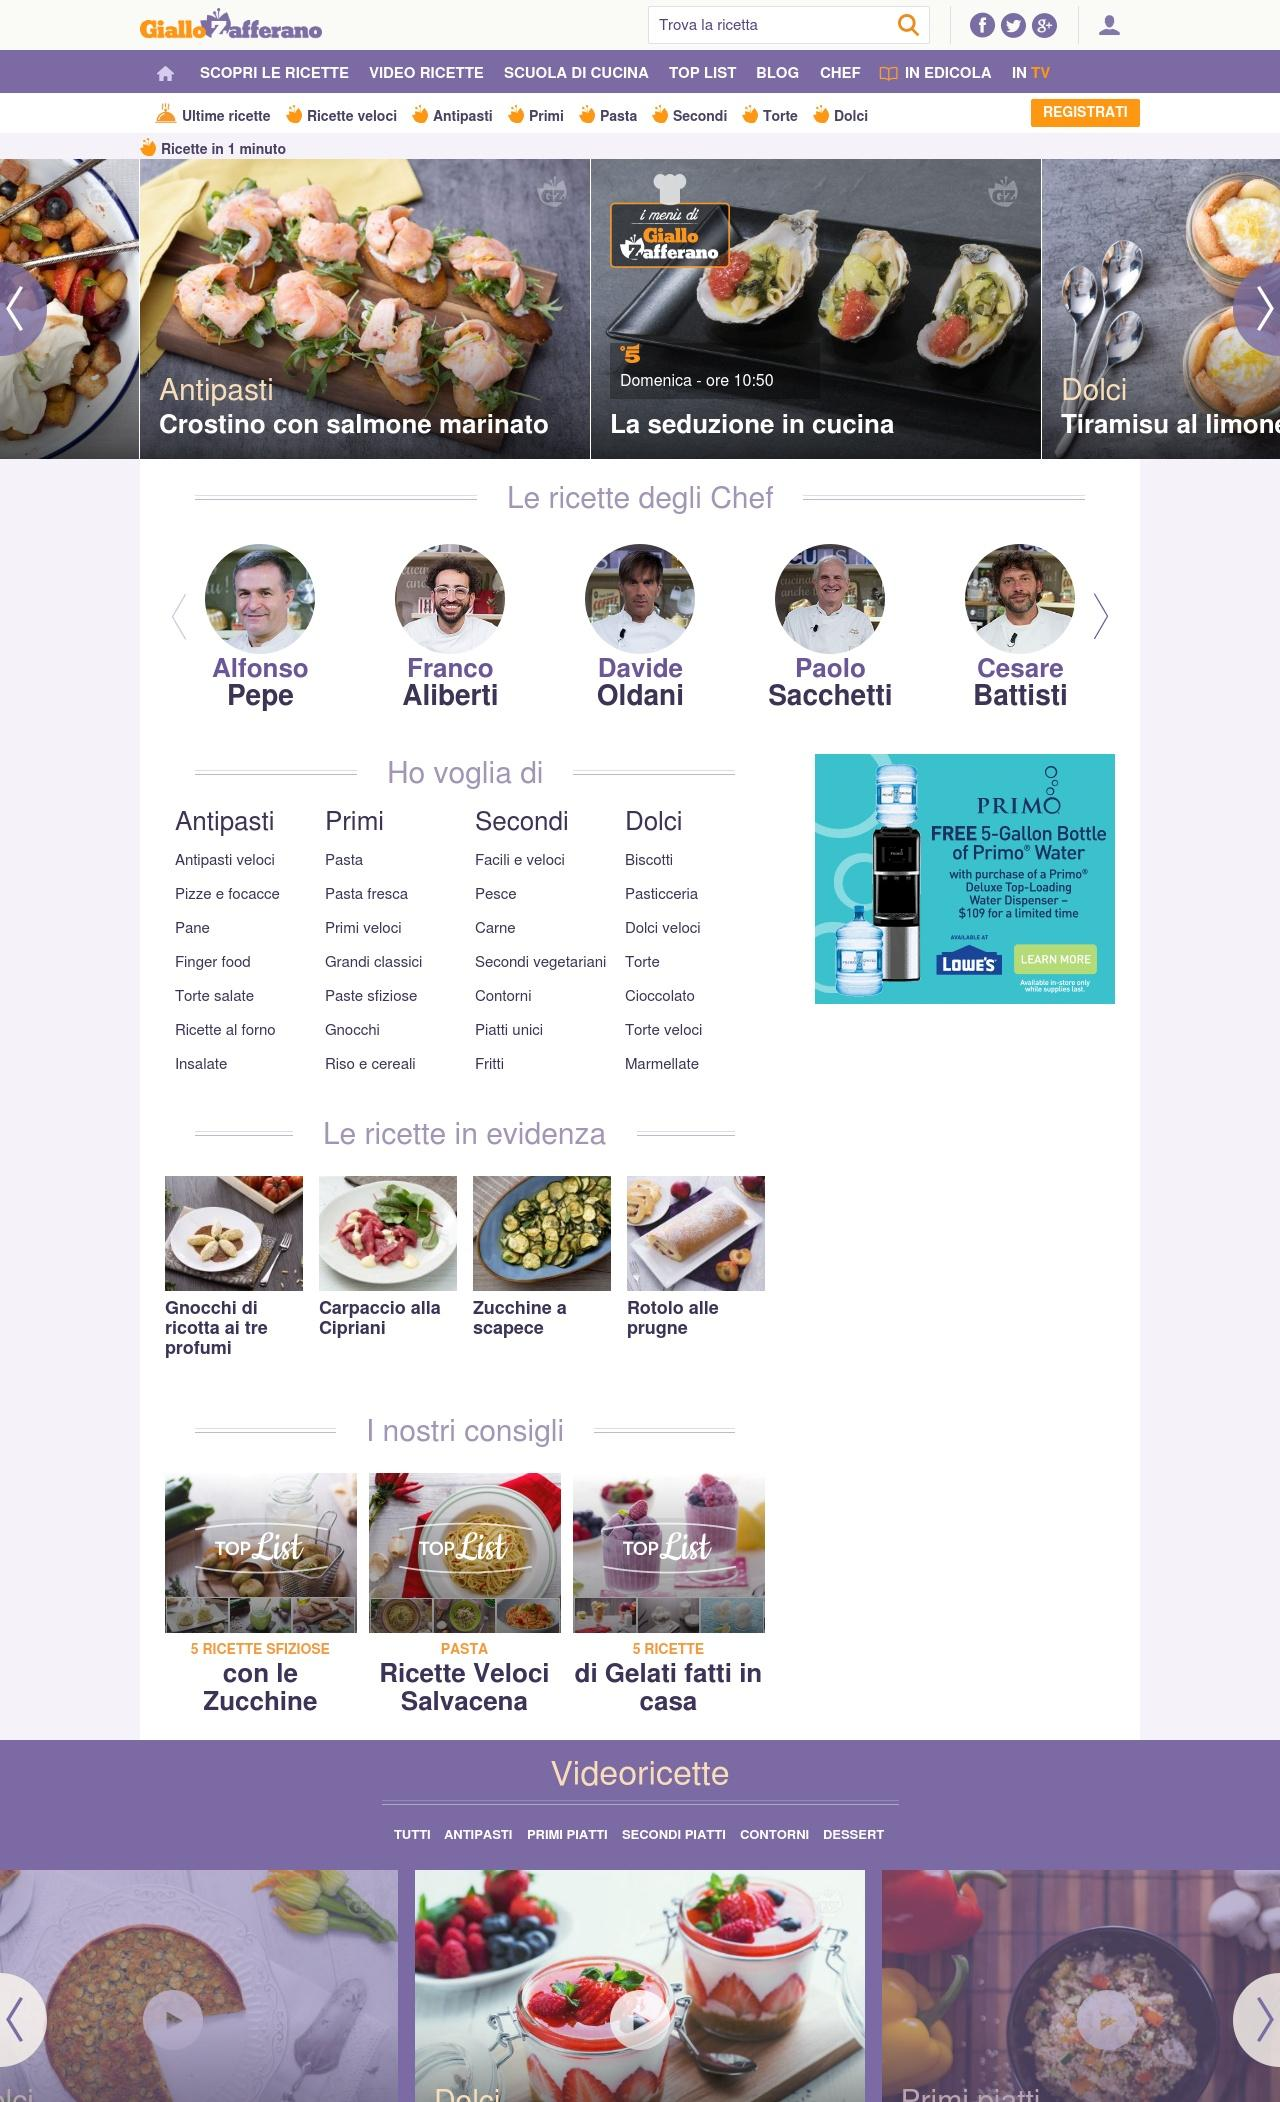
\includegraphics[scale=0.1]{images/homepage/homepage-1.jpeg}
		\subcaption{}
	\end{subfigure}
	\begin{subfigure}[b]{0.3\textwidth}
		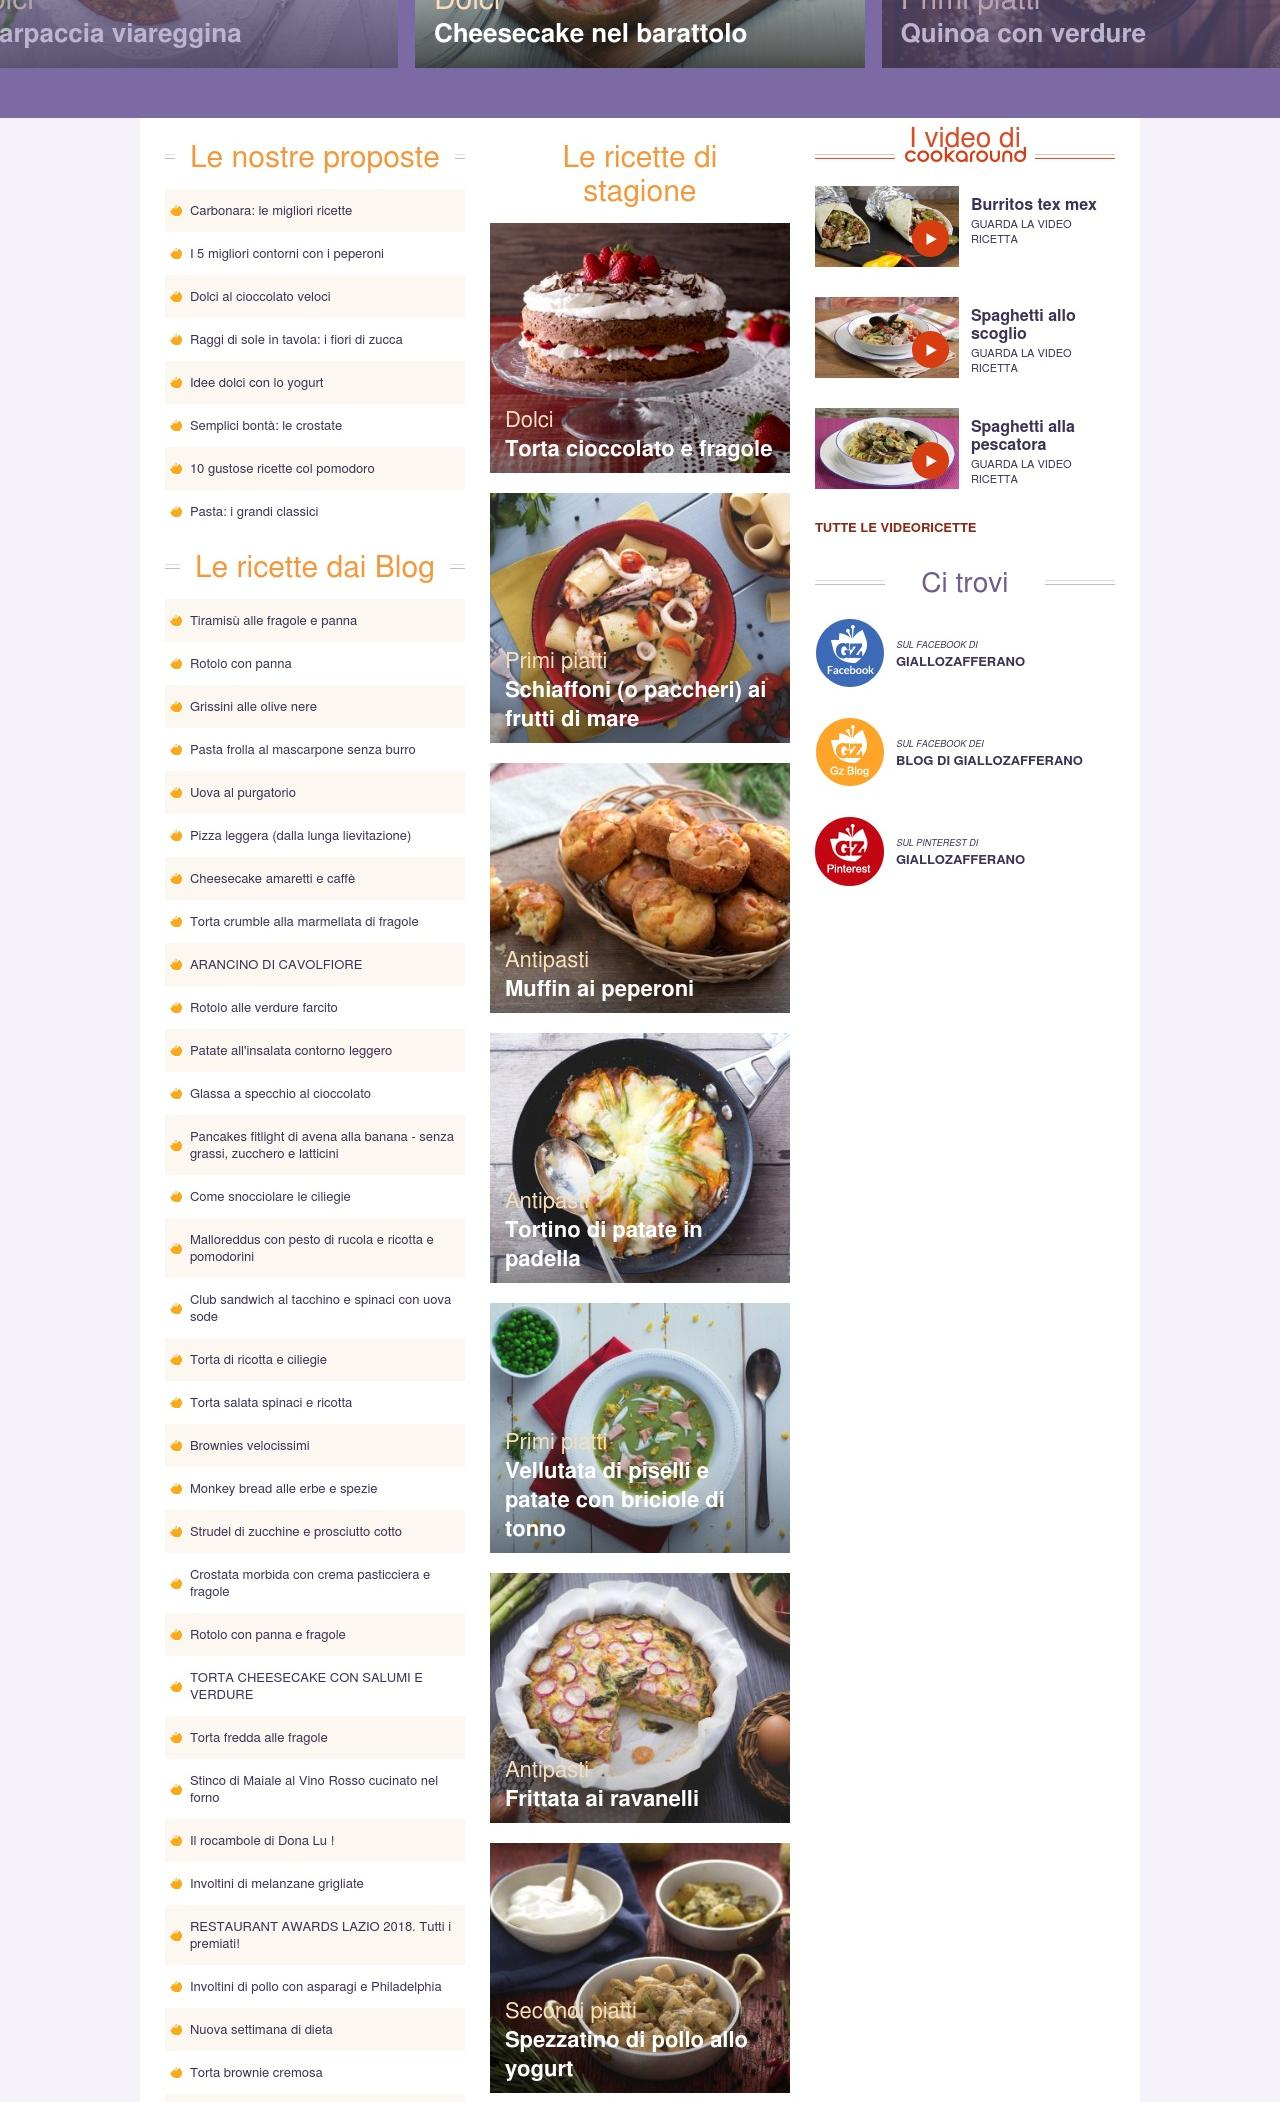
\includegraphics[scale=0.1]{images/homepage/homepage-2.jpeg}
		\subcaption{}
	\end{subfigure}
	\begin{subfigure}[b]{0.3\textwidth}
		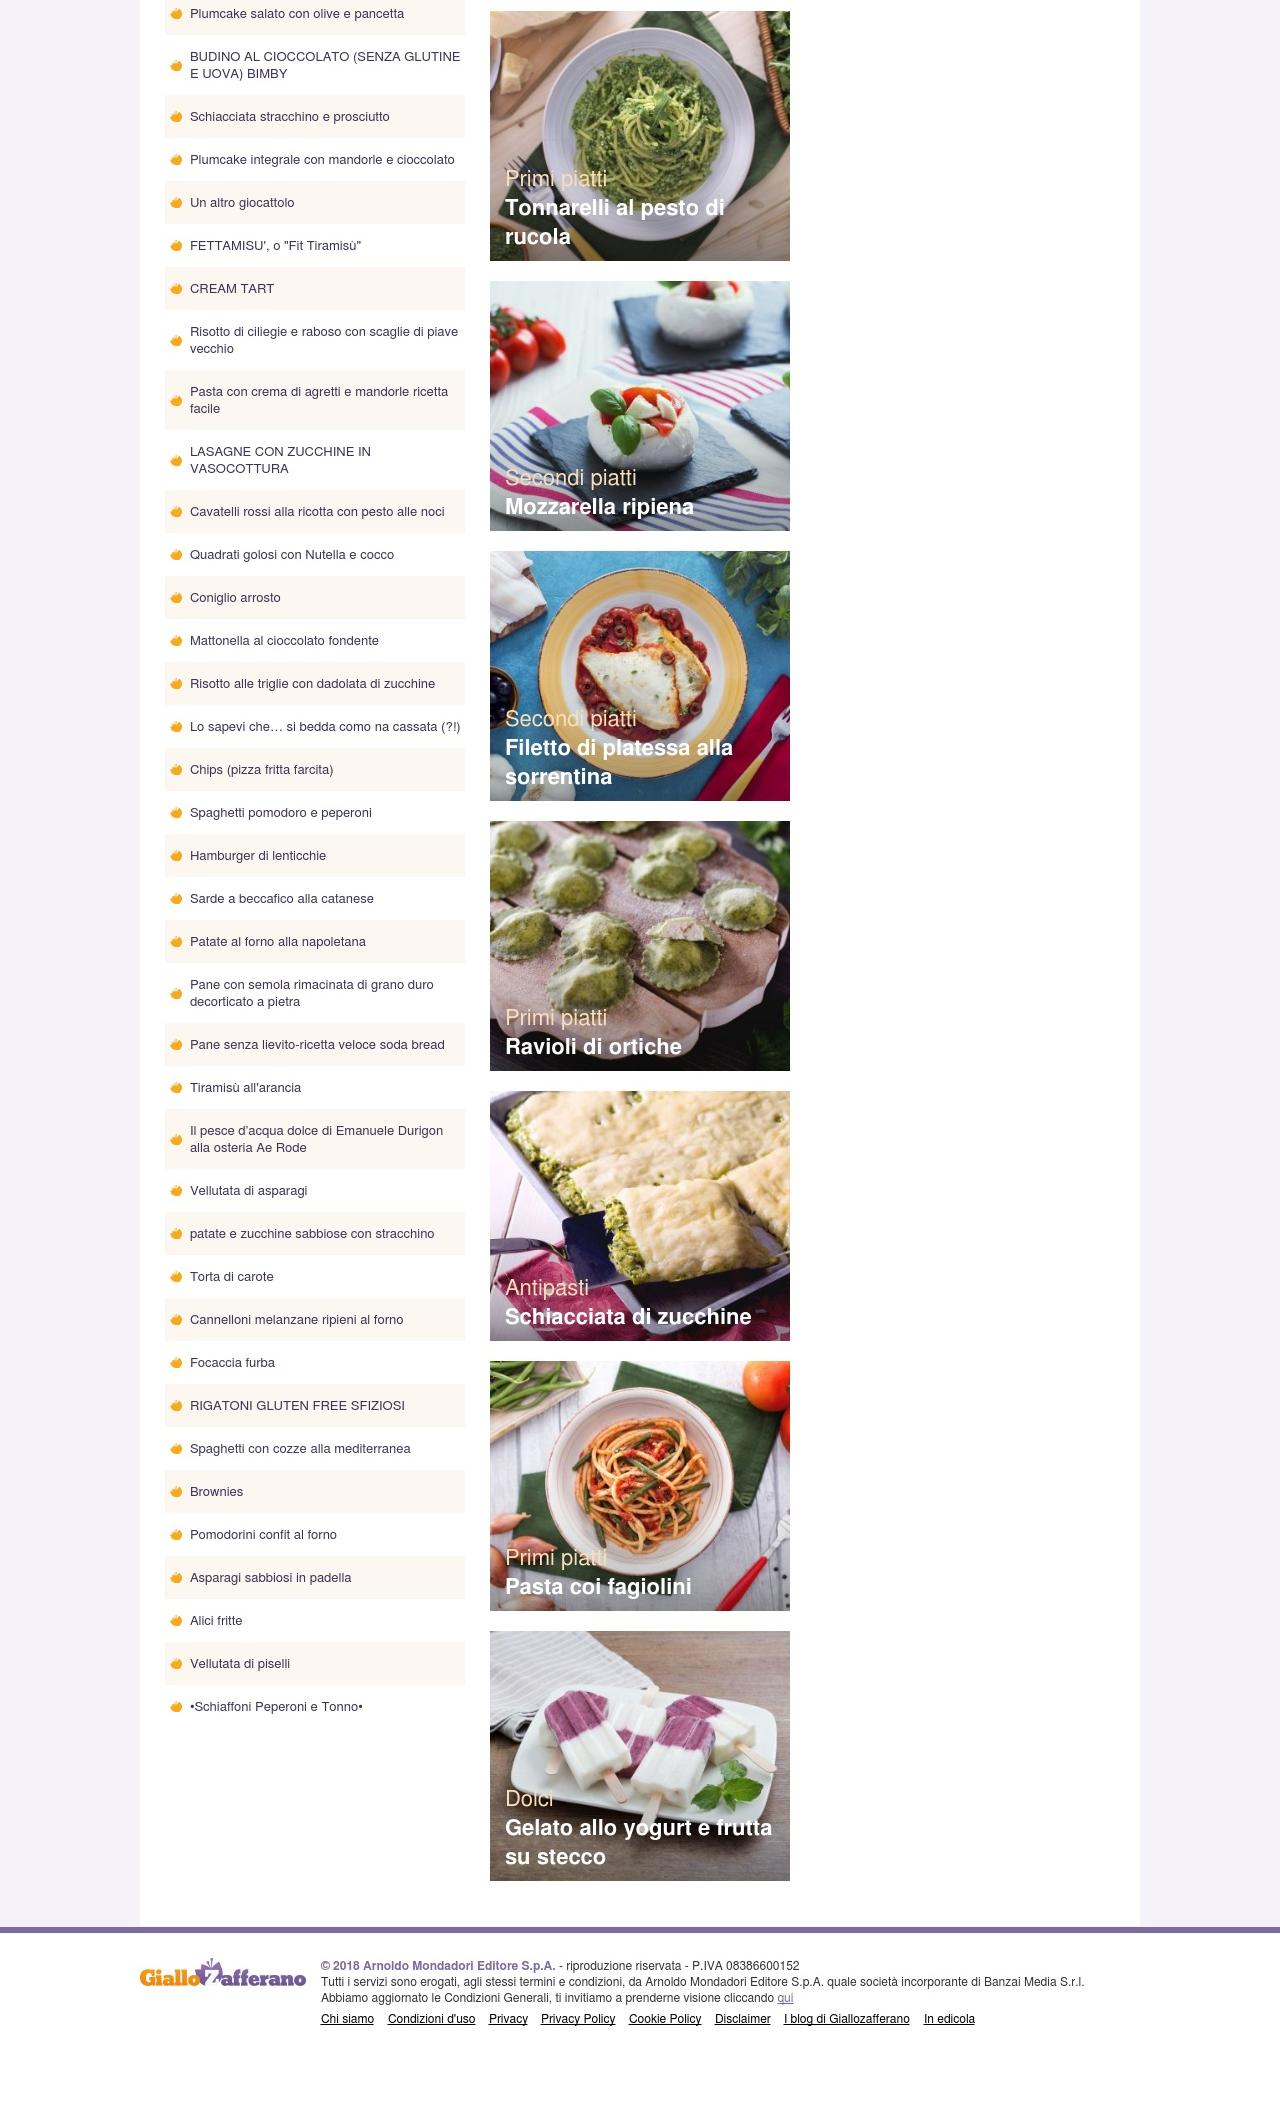
\includegraphics[scale=0.1]{images/homepage/homepage-3.jpeg}
		\subcaption{}
	\end{subfigure}
	\caption{Homepage (homepage-1,2,3.png) - https://www.giallozafferano.it}
	\label{fig:homepage}
\end{figure}


\subsection{Considerazioni generali}
L'homepage sta ad un sito web come la vetrina sta ad un negozio: essa ha infatti un ruolo introduttivo unico, in cui l'informazione deve essere fruibile nel modo più efficace possibile. Un buon design della homepage deve tener conto di quattro elementi principali:
\begin{itemize}
	\item Identità, del sito stesso o della compagnia/persona che rappresenta;
	\item Navigazione;
	\item Tempestività ed attenzione al contenuto;
	\item Strumenti, come la ricerca.
\end{itemize}
Il modo in cui l'importanza di questi elementi viene pesata dipende molto dalla natura del sito; l'homepage di giallozafferano è dominata dalla navigazione verso i contenuti : si vede subito come i riferimenti alle varie categorie di ricette siano disponibili immediatamente, sia nella barra di navigazione che nel corpo vero e proprio.

\subsection{Le 6 W}
Al fine di valutare come l'informazione viene presentata, si farà riferimento ai 6 assi informativi: Where, Who, Why, What, When, How; essi devono essere dati all'utente nel minor tempo possibile.

\subsubsection{Where} 

Domanda: \textit{"A quale sito sono arrivato? Che tipo di contenuto mi offre?"}

Come detto in precedenza, già nell'homepage notiamo una forte attenzione ai contenuti. Ciò è molto utile ad un utente che arriva per la prima volta nel sito, in quanto sin da subito capisce che si tratta di un sito collegato alla cucina; è probabile però che a primo impatto si possa pensare di essere arrivati nel sito di un ristorante: l'utilizzo di uno slide di immagini che occupa più della metà della parte superiore della pagina presenta foto di cibi, senza alcun riferimento al fatto che rimandano alla ricetta di quel piatto. Solo dopo aver superato l'impatto grafico iniziale, ci si accorge della parola \textit{ricette} che ricorre più volte, e si realizza di essere arrivati in un sito di ricette culinarie. 
Altro elemento che fa capire di essere in un sito il cui tema è la cucina è il nome, posto correttamente nell'angolo superiore sinistro della pagina (punto d'entrata della visualizzazione della pagina), nel quale \textbf{zafferano} richiama l'ingrediente principale del famoso risotto alla milanese.

\begin{figure}[h!]
	\centerline{
	
\includegraphics[scale=0.25]{images/homepage/header.png}}
	\caption{Header con logo (header.png)}
\end{figure}


\subsubsection{Who} 

Domanda: \textit{"Chi c'è dietro questo sito?"}

L'identità del creatore/possessore del sito non risulta totalmente chiara: sicuramente la presenza ben visibile del logo aiuta ad identificarlo se già lo si conosce, tuttavia per un utente che non ha mai sentito parlare del sito l'autore risulta ignoto e probabilmente rimarrà tale; in effetti, per trovare alcune informazioni a riguardo, è necessario scorrere fino alla fine della pagina (che come detto in precedenza è troppo lunga), fino ad arrivare nel footer, dove è scritto con un carattere molto piccolo il proprietario, \textit{Arnoldo Mondadori Editore S.p.A.}, al di sotto del quale è poi presente un link \textit{Chi siamo}, che porta ad una pagina che offre alcune informazioni aggiuntive riguardo non solo l'azienda, ma anche il team che lavora per il sito.
In sintesi dunque l'asse who non è ben specificato, poiché richiede troppo tempo per trovare risposta, cosa che l'utente non ha e che può portare ad un aumento dell'insoddisfazione.

\begin{figure}[h!]
	\centerline{
	
\includegraphics[scale=0.25]{images/homepage/footer.png}}
	\caption{Footer (footer.png)}
\end{figure}

\begin{figure}[h!]
	\centerline{
	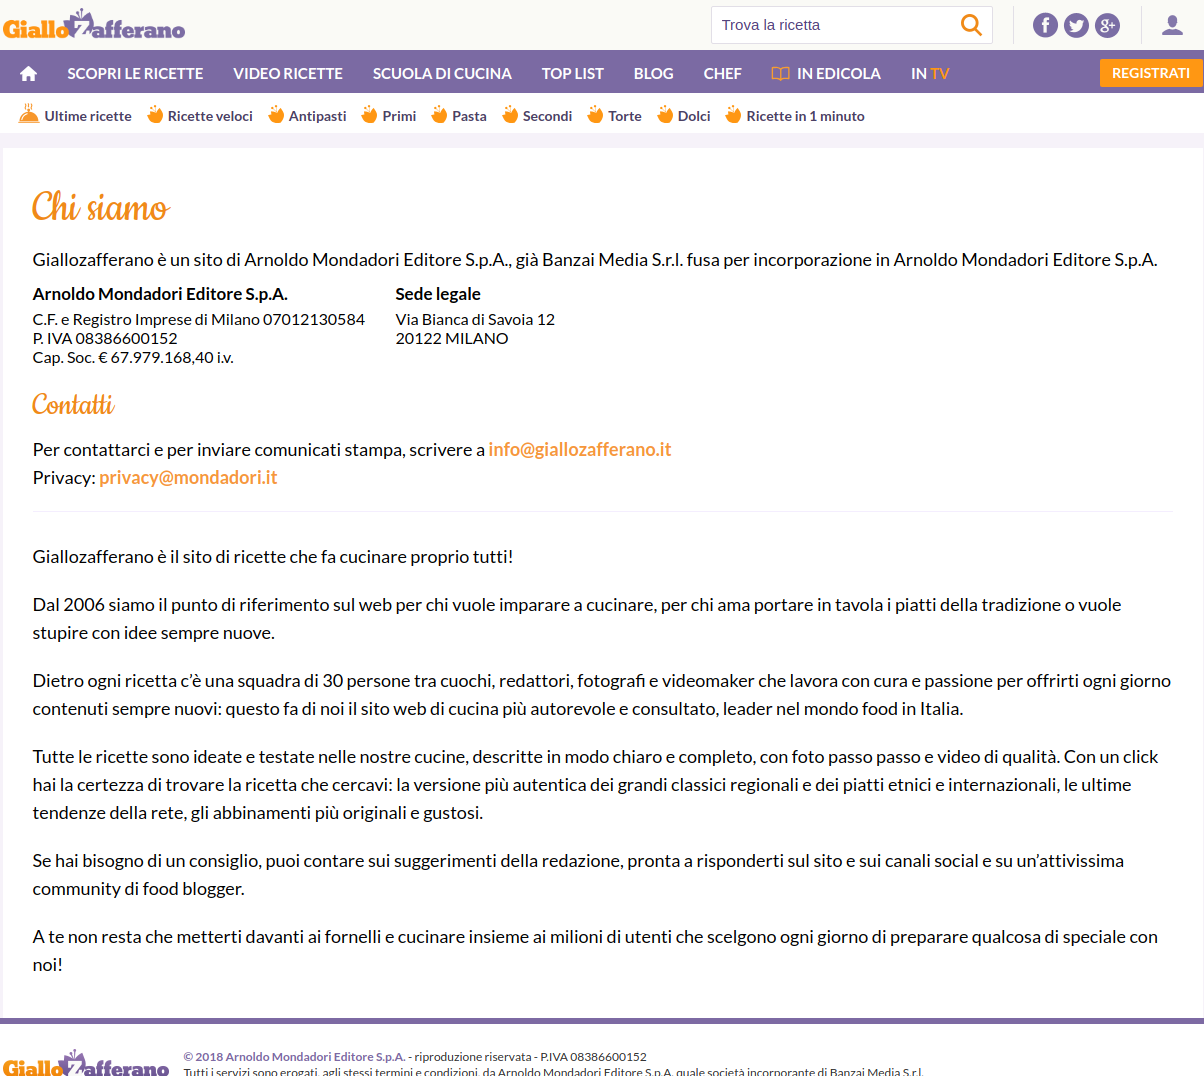
\includegraphics[scale=0.25]{images/chi-siamo.png}}
	\caption{Pagina "chi siamo" (chi-siamo.png) \newline- www.giallozafferano.it/staff/chisiamo.html}
\end{figure}

\newpage

\subsubsection{Why} 

Domanda: \textit{"Perché dovrei rimanere nel sito? Che benefici mi offre?"}

Il sito non dà esplicitamente dei motivi per cui un utente dovrebbe rimanerci, probabilmente perché si basa molto sulla propria fama (come specificato nell'analisi preliminare, esso è tra i più visitati al mondo nel settore cibo). Nonostante la fama conti, però, non è vantaggioso basarsi solo su di essa: nel web navigano persone con capacità e conoscenze diverse che il sito deve essere in grado di accogliere e "tenere" nel maggior numero possibile; ad esempio, un utente che non ha mai cercato ricette di cucina, potrebbe decidere di lasciare il sito perché non esperto del settore e perché non è in grado di valutare in breve tempo la qualità e l'affidabilità di giallozafferano, nonostante le numerose sezioni e i richiami agli chef che propone nella home. Per aumentare l'attrattiva, basterebbe un breve paragrafo di testo in cui esaltare i motivi del successo del sito, come ad esempio ciò che è scritto nella pagina "Chi siamo".

\newpage

\subsubsection{What} 

Domanda: \textit{"Che cosa offre il sito?"}

Come già detto, l'homepage è fortemente orientata al contenuto, che viene proposto più volte ed in maniera diversa. Il menù di navigazione (quello più in alto) principale presenta diverse voci che richiamano ciò che offre il sito, cioè le ricette, tuttavia è costituito da elementi poco chiari ed è necessario passarci sopra con il mouse per capire meglio a cosa portano. La presenza ricorrente della parola \textit{ricette}, in tutta la home, dà un'ulteriore conferma del contenuto del sito, assieme al sottomenù ed agli elenchi nella sezione \textit{Ho voglia di} (purtroppo tagliati in uno schermo con risoluzione 1920x1080, come si vede in \ref{fig:home_primo_pezzo}), i quali però richiamano parte del secondo menù di navigazione, il che ancora una volta rischia di creare confusione. 

\begin{figure}[h!]
	\centerline{
	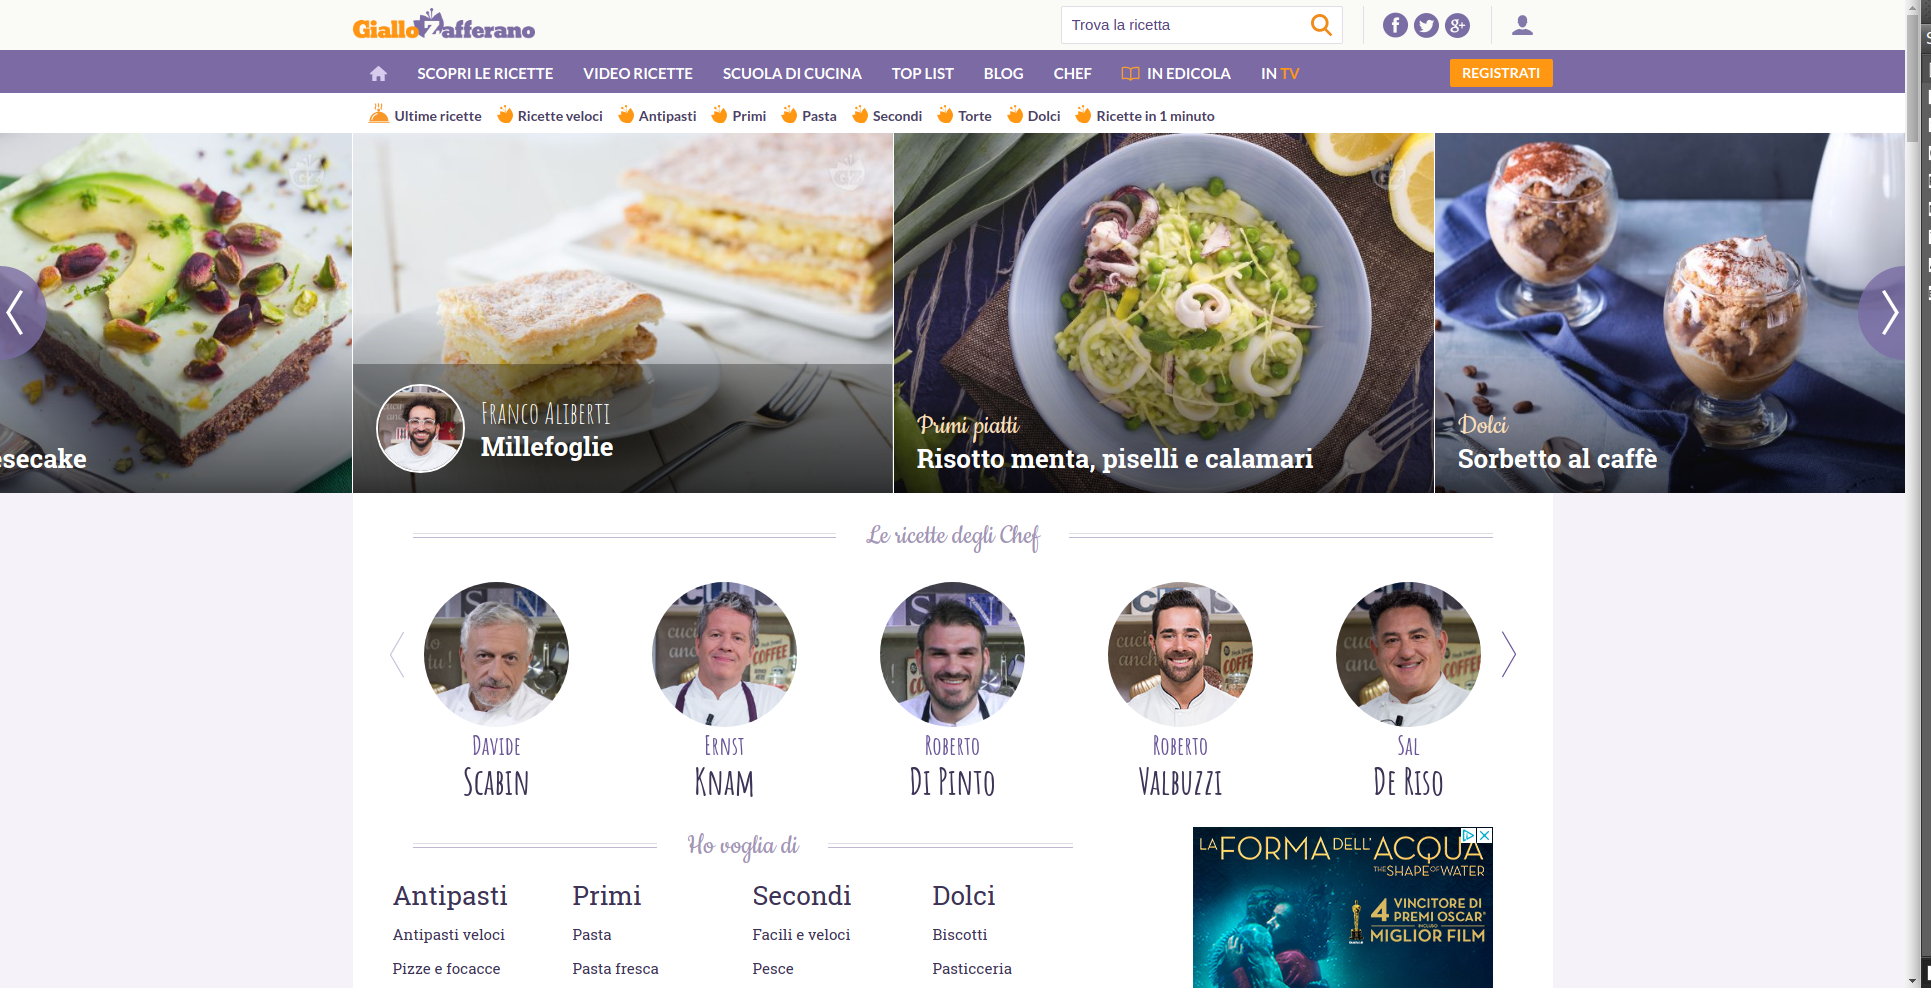
\includegraphics[scale=0.25]{images/home_primo_pezzo.png}}
	\caption{Homepage, prima schermata (home\textunderscore primo\textunderscore pezzo.png)}
	\label{fig:home_primo_pezzo}
\end{figure}


\subsubsection{When} 
\label{subsez:when}

Domanda: \textit{"Ciò che mi offre il sito è nuovo/aggiornato?"}

La homepage non dà alcun riferimento temporale. L'unica indicazione di novità sta nel secondo menù, nel quale compare la voce \textit{Ultime ricette} (vedi \ref{fig:secondo_menu}). Essa però non basta a dare un senso di aggiornamento continuo e novità al sito, è un elemento statico che non cambia nel tempo; cliccandoci sopra, inoltre, si arriva ad una pagina in cui vengono elencate le ultime ricette, senza però fornire alcuna data: l'intero sito dunque non riesce a soddisfare quest'asse sufficientemente.

\newpage

\subsubsection{How} 

Domanda: \textit{"Ho capito cosa mi offre. Come faccio ad arrivare a ciò che mi interessa?"}

La home fornisce diverse strade per raggiungere il contenuto, il che è un pregio, tuttavia sono disposte in modo confusionario; di seguito vengono analizzati in dettaglio i macro-componenti che racchiudono questi percorsi.

\paragraph{Primo menù di navigazione}
Il primo menù è abbastanza visibile ed è posto in alto, miglior posizione possibile. Le voci sono scritte in maiuscolo, cosa che diminuisce di circa il 10\% la leggibilità data la poca abitudine dell'utente medio a leggerlo.

\begin{figure}[h!]
	\centerline{
	
\includegraphics[scale=0.5]{images/primo_menu.png}}
	\caption{Primo menù di navigazione(primo\textunderscore menu.png)}
	\label{fig:primo_menu}
\end{figure}

\subparagraph{Voci}
\begin{itemize}
	\item \textbf{SCOPRI LE RICETTE} rimanda ad una pagina contenente tutte le ricette presenti nel sito divise per portata ed ha un sottomenù le cui voci sono le varie portate e rimandano alla stessa pagina, in cui però le ricette sono già filtrate in base alla voce scelta.
	\item \textbf{VIDEO RICETTE} ha un sottomenù identico al precedente e rimanda ad una pagina contente tutte le ricette aventi oltre ad una descrizione scritta, un video, divise per portata. Il fatto che questi primi due link rimandino ad una pagina così simile può però confondere l'utente, che potrebbe aspettarsi pagine completamente diverse: al momento dell'analisi, invece, le pagine risultano perfettamente identiche, le stesse ricette sono presentate in entrambe. In effetti ci si accorge che \textit{VIDEO RICETTE} non è una pagina a parte, bensì una sotto-pagina di \textit{SCOPRI LE RICETTE}! Personalmente dunque ritengo la scelta di riservarvi una voce di menù controproducente, sarebbe meglio invece usarla come filtro di ricerca o come voce del sottomenù di \textit{SCOPRI LE RICETTE};
	\item \textbf{SCUOLA DI CUCINA} è un'altra voce che può creare confusione: l'insegnamento della cucina non comprende anche le ricette? Solo passandoci sopra  con il mouse e facendo comparire il sottomenù ci si accorge che sono comprese solo tecniche e ricette "generali", cioè non legate ad uno specifico piatto, come ad esempio pulire la verdura,  preparare salse basilari ecc...
	\item \textbf{TOP LIST}: ancora una volta non è ben chiaro a cosa si riferisca la voce; innanzitutto l'utilizzo dell'inglese non è appropriato in un sito italiano, soprattutto considerando la grande varietà di utenti a cui si rivolge: ad esempio, molto probabilmente un anziano non ha idea di cosa voglia dire di preciso. 
	Comunque, anche ammesso che un utente conosca l'inglese, tale voce rimane vaga: lista dei migliori? E' intuibile che ci si sta riferendo alle migliori ricette, ma non è assolutamente banale.
	\item \textbf{BLOG} rimanda al blog collegato al sito (ma esterno), come ci si aspetta.
	\item \textbf{CHEF} rimanda alla pagina delle ricette ideate dagli chef che lavorano per il sito, mentre ci si aspetterebbe un semplice elenco di essi.
	\item \textbf{IN EDICOLA} rimanda ad una pagina informativa riguaro la rivista collegata al sito, come ci si aspetta.
	\item \textbf{IN TV} rimanda ad una pagina il cui titolo è \textit{"I menù di giallozafferano"}, la cui natura è inaspettata e non molto chiara; probabilmente infatti un utente si aspetta di trovare una pagina informativa come quella a cui rimanda la voce precedente, invece trova dei contenuti totalmente diversi sia strutturalmente che concettualmente.
\end{itemize}


\subparagraph{Sottomenù}

Le prime tre voci del menù appena descritto hanno un comportamento dinamico: quando il cursore ci passa sopra, compare un sottomenù: il fatto che ciò accada con solo una parte delle voci è un difetto, in quanto rende la struttura del menù poco prevedibile. In ogni caso, i sottomenù a tendina sono facilmente navigabili, in quanto viene lasciato un margine abbastanza ampio tra la parola e la dimensione effettiva del pulsante; il fatto che si espandano verticalmente inoltre è una buona cosa e da preferire rispetto ad un elenco orizzontale. Un difetto è il non essere \textit{fault tollerant}, cioè non appena il cursore esce dal sottomenù, questo scompare.


\begin{figure}[h!]
	\centering
	\begin{subfigure}[b]{0.3\textwidth}
		
\includegraphics[scale=0.5]{images/sottomenu-1.png}
		\subcaption{}
	\end{subfigure}
	\begin{subfigure}[b]{0.3\textwidth}
		
\includegraphics[scale=0.5]{images/sottomenu-2.png}
		\subcaption{}
	\end{subfigure}
	\begin{subfigure}[b]{0.3\textwidth}
		
\includegraphics[scale=0.5]{images/sottomenu-3.png}
		\subcaption{}
	\end{subfigure}
	\caption{I 3 sottomenù (sottomenu-1.png, sottomenu-2.png, sottomenu-3.png)}
\end{figure}



\paragraph{Secondo menù di navigazione}

Il secondo menù è posto appena sotto il primo e riporta molti riferimenti già definiti in precedenza.

\begin{figure}[h!]
	\centerline{
	
\includegraphics[scale=0.5]{images/secondo-menu.png}}
	\caption{Secondo menù di navigazione (secondo-menu.png)}
	\label{fig:secondo_menu}
\end{figure}

\subparagraph{Voci}

\begin{itemize}
	\item \textbf{Ultime ricette} Come detto in \ref{subsez:when}, rimanda alla pagina con le ultime ricette.
	\item \textbf{Ricette veloci - Antipasti - Primi - Pasta - Secondi - Torte - Dolci} Si comportano come le voci dei sottomenù delle prime due voci del primo menù di navigazione, quindi rimandano alla pagina delle ricette, visualizzando solo la categoria scelta: si riconferma la ridondanza e la conseguente confusione di link ripetuti inutilmente.
	\item \textbf{Ricette in un minuto} Tale voce ha un comportamento completamente diverso dalle altre: rimanda alla pagina https://funtip.giallozafferano.it/, che si presenta totalmente diversa dalle altre, senza alcun menù di navigazione, ad esempio.
\end{itemize}

\paragraph{Riferimenti nel corpo}

L'intero contenuto della pagina presenta ulteriori link a categorie di ricette o ricette singole. Precisamente, ci sono 9 componenti diverse che li racchiudono, che tuttavia ometto di descrivere in quanto vale quello che è stato detto per i vari menù, cioè il fatto che creano solamente un senso di confusione e ridondanza
(sono visibili nella figura \ref{fig:homepage}, nel corpo della pagina).



\section{Contenuto}
Dopo aver esaminato la \textit{vetrina} del sito passiamo ora all'analisi del contenuto. In particolare, si analizzerà la pagina di una ricetta/tecnica di cucina, in quanto è la tipologia di pagina più significativa, più numerosa e sicuramente più visitata (forse dopo la home), dato che l'obiettivo principale del sito è offrire ricette; oltre ad essa, verrà analizzata brevemente la pagina 404 ed infine anche la tipologia di pagina il cui scopo è elencare le ricette, ma nella sezione \ref{sez:ricerca}. Per esse l'analisi sarà leggermente diversa rispetto a quella effettuata per la home, in quanto l'importanza degli assi informativi cambia.

\subsection{Pagina di una ricetta}
\subsubsection{Descrizione generale}
\label{subsez:ricetta-descr}
Prenderò come esempio la pagina relativa alla (video)ricetta della parmigiana di melanzane, al link \url{https://ricette.giallozafferano.it/Parmigiana-di-melanzane.html}.
La pagina si presenta molto lunga, 22 scroll e mezzo verticali su uno schermo con risoluzione 1920x1080, con il browser in modalità non massimizzata: è un numero troppo elevato, considerando che circa solo il 42\% degli utenti fa uso di scroll nelle pagine interne; tuttavia è da considerare anche il livello di interesse dell'utente, il quale probabilmente è arrivato nella pagina perché veramente interessato ad imparare la ricetta e dunque abbastanza propenso a scrollare, pur di ricevere le informazioni che desidera.
\\~Ogni area di testo è accompagnata da un titolo descrittivo, cosa che aiuta molto il lettore: esso è però scritto in corsivo, cosa che aiuta sì il contrasto, ma diminuisce la leggibilità. 
\\~Come si può vedere in figura \ref{fig:ricetta-1}, al momento dell'ingresso nella pagina le informazioni sono quasi nulle: c'è il titolo della ricetta, il voto che gli utenti le hanno dato ed il video (solo nel caso delle video ricette, negli altri casi è presente un'immagine del piatto della stessa dimensione). Più sotto poi si intravedono le parole \textit{Difficoltà:}, \textit{Preparazione}, \textit{Cottura}, \textit{Dosi per}, \textit{Costo}: il fatto che siano tagliate può incoraggiare l'utente a fare scroll per vedere cosa c'è effettivamente sotto, il che è una buona cosa (se non le vedesse affatto sarebbe ignaro del fatto che la pagina continua). 
~\\C'è poi una cosa che rischia di creare fastidio nell'utente: nel momento in cui la pagina viene caricata, la video ricetta parte in automatico; nonostante l'audio sia di default disattivato, la cosa può stressare l'utente perché non richiesta esplicitamente. Inoltre, non appena si fa uno scroll che supera la posizione del video, esso viene spostato in basso a destra, senza venire messo in pausa: se l'utente vuole leggere la ricetta mentre guarda il video per avere delle informazioni più dettagliate può trarne beneficio, ma lasciarlo sotto gli occhi di un utente che non vi è interessato contribuisce solamente ad aumentarne lo stress e la voglia di andarsene.
~\\Come ultima cosa, vediamo che anche dopo aver fatto dello scroll, la barra superiore in cui sono contenuti logo, ricerca e collegamenti ai social, rimane staticamente attaccata alla parte alta dello schermo, comprendo informazioni potenzialmente utili.

\begin{figure}[h!]
	\centerline{
	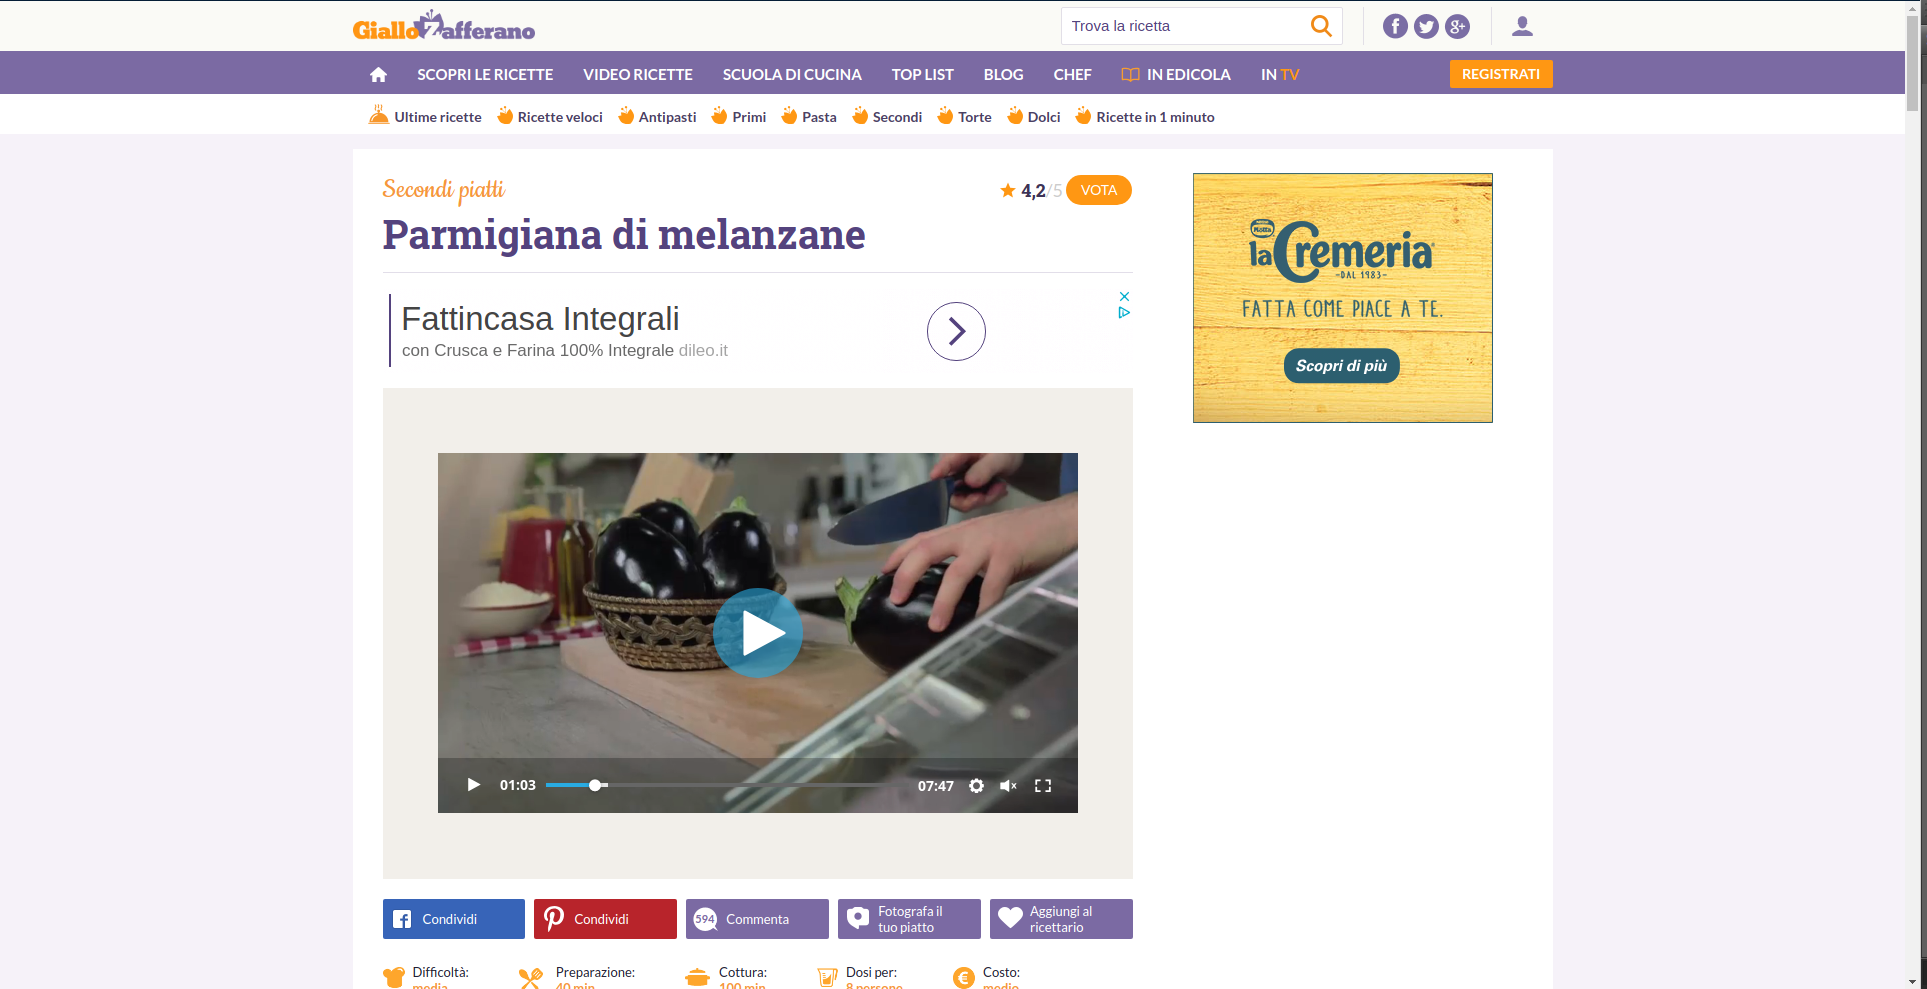
\includegraphics[scale=0.2]{images/ricetta-1.png}}
	\caption{Prima schermata della pagina ricetta della parmigiana di melanzane (ricetta-1.png) - \newline https://ricette.giallozafferano.it/Parmigiana-di-melanzane.html}
	\label{fig:ricetta-1}
\end{figure}

\newpage

\subsubsection{Le 6 W}

\paragraph{Where} 
Tale asse continua ad avere molta importanza nelle pagine interne poiché risolve il problema del \textit{lost in navigation}, permettendo di rendere chiaro all'utente il contesto in cui si trova. Dato che nel web non c'è il senso del movimento nè della bussola, utilizzare un collegamento alla home dà un orientamento "verso casa"; ciò viene fatto all'interno della pagina attraverso il logo/nome in alto a sinistra, tuttavia non è sufficiente, poiché se un utente è arrivato nella pagina attraverso il \textit{deep linking}, dargli come riferimento solo il link alla home costituisce un click sprecato e lo costringe a spostarsi dal luogo in cui c'è l'informazione di suo interesse. 
L'uso di bradcrumb avrebbe comunicato efficacemente gran parte dell'asse where, ma l'unico accenno di esso sono le parole \textit{Secondi piatti}, poste sopra al titolo della ricetta: esse sono un link che rimanda alla pagina delle ricette della categoria secondi piatti, il che può aiutare l'utente a capire parte del percorso che porta alla pagina in analisi, ma è ancora una volta un click sprecato che costringe l'utente a spostarsi.
In sostanza dunque nonostante i percorsi di navigazione siano nella home ben segnalati, rimangono difficili da ricordare una volta arrivati all'informazione ricercata.
\begin{comment}
Per non affaticare ulteriormente il visitatore ed aiutarlo a tenere a mente i percorsi fatti sarebbe stato poi opportuno colorare diversamente i link già visitati, dato che è una convenzione non standard riconosciuta in tutto il web.
\end{comment}

\paragraph{Who} 
 Anche quest'asse rimane obbligatorio nelle pagine interne, ma è sufficiente esporre il logo del sito/azienda, cosa che giallozafferano fa mantenendolo in alto a sinistra.
 
\paragraph{Why} 
L'asse why diventa nelle pagine interne opzionale ma consigliato. Come per la homepage, anche nella pagina di una ricetta esso non trova risposta, nonostante basterebbe una breve descrizione o uno slogan.

\paragraph{What} 
Tale asse rimane obbligatorio e valgono per la pagina le considerazioni fatte per la home: la presenza di riferimenti al cibo e alle ricette in tutta la pagina fanno capire che il tema è la cucina ed il titolo della ricetta aiuta a capire di essere nella pagina specifica di un piatto, anche se un utente potrebbe pensare che sia solo una pagina che descrive l'alimento e non effettivamente le procedure per la sua preparazione.

\paragraph{When}
L'asse when è opzionale e viene comunicato nello stesso modo in cui era comunicato nella home, cioè attraverso il link \textit{Ultime ricette} nel secondo menù di navigazione. 

\paragraph{How} 
Quest'asse è opzionale ma consigliato e viene solitamente soddisfatto fornendo una funzionalità di search, cosa che il sito offre posizionandola correttamente in alto a destra e anche in basso, alla fine della pagina, prima del footer.
\clearpage

\subsubsection{Schermate}
Dato che la pagina è molto lunga, la si analizzerà per schermate, a partire da quella successiva alla prima, che è già stata descritta in \ref{subsez:ricetta-descr} I blocchi di testo successivi si riferiranno sempre all'immagine sopra di loro. 


\begin{figure}[h!]
	\centerline{
	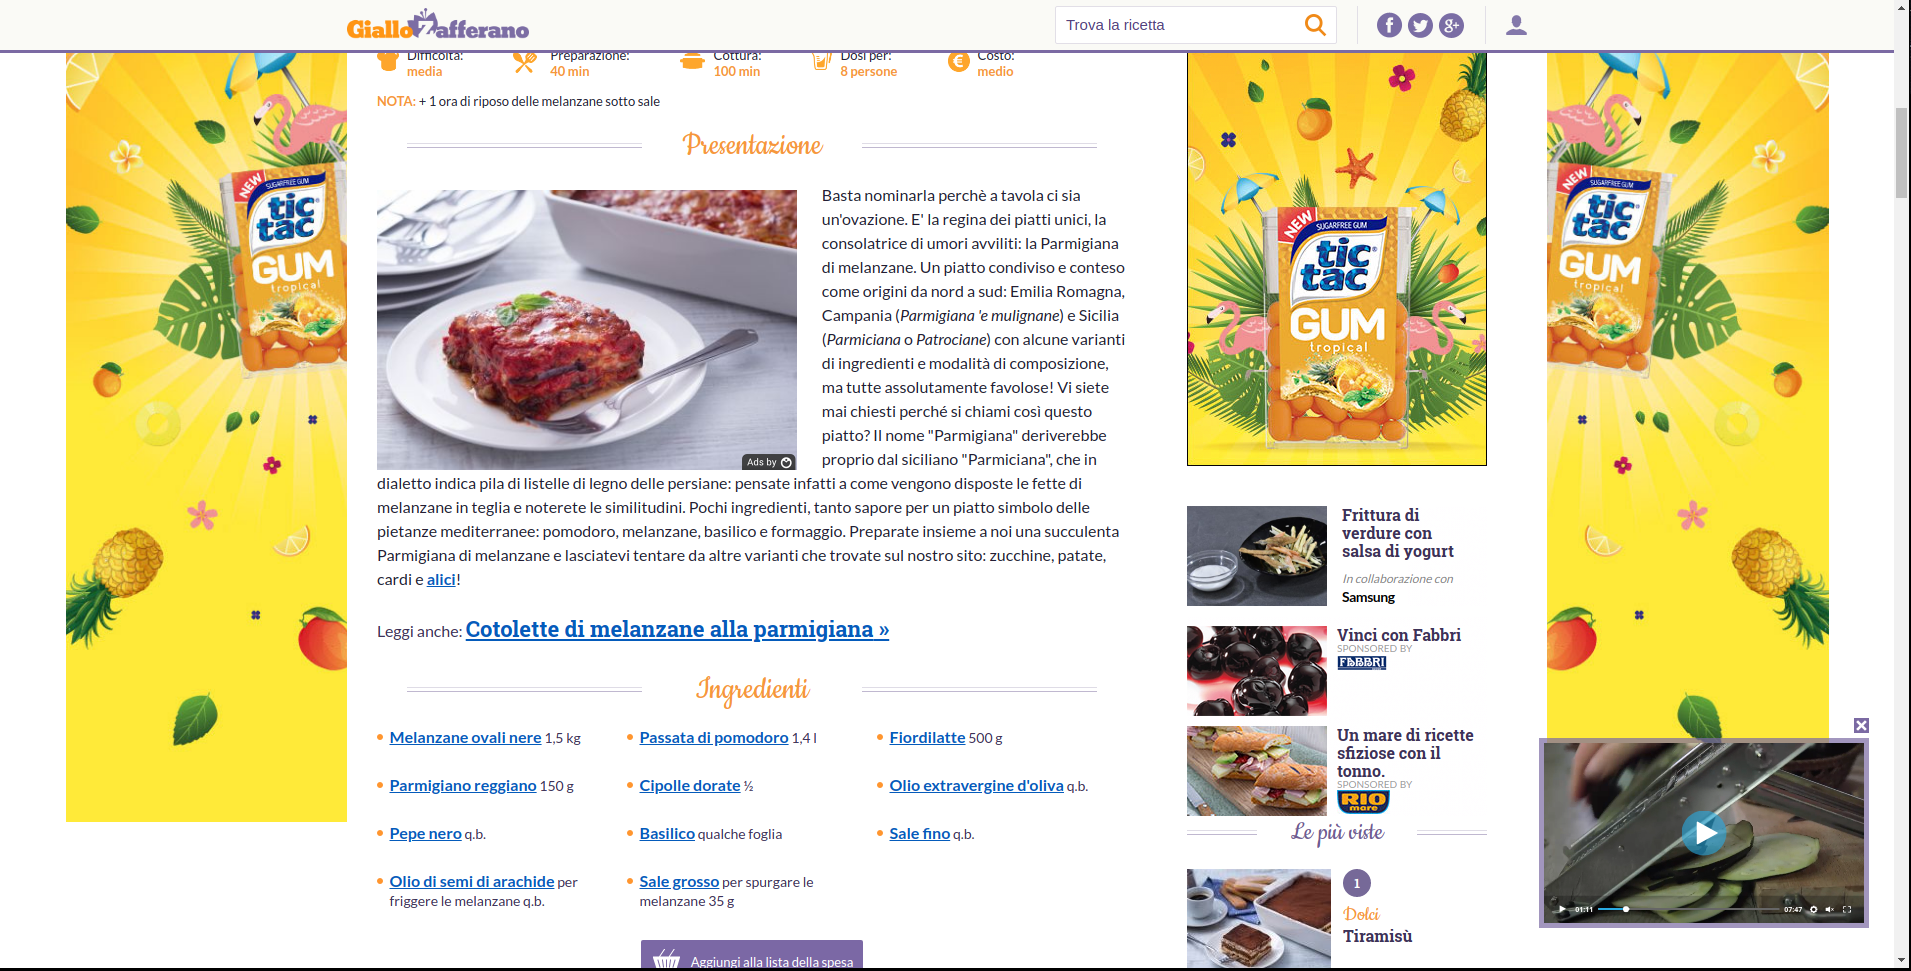
\includegraphics[scale=0.2]{images/ricetta-2.png}}
	\caption{Seconda schermata della pagina ricetta della parmigiana di melanzane (ricetta-2.png)-\newline https://ricette.giallozafferano.it/Parmigiana-di-melanzane.html}
	\label{fig:ricetta-2}
\end{figure}

In questa parte troviamo come prima cosa la \textit{Presentazione} della ricetta con solitamente una contestualizzazione storica, accompagnata da un'immagine; quest'ultima è abbastanza grande da attirare l'attenzione dell'utente, tuttavia non è cliccabile: solitamente le immagini hanno un tasso di click superiore al testo, dunque sarebbe opportuno renderla cliccabile, avendo come evento anche semplicemente l'ingrandimento della foto, per evitare che utenti inesperti perdano tempo nell'attesa di un redirect che non arriverà mai.
Per quanto riguarda il testo, anch'esso ha bisogno di miglioramenti: innanzitutto andrebbe posizionato a sinistra della foto, in modo da esaltarne l'importanza; poi andrebbe disposto in blocchi facendo uso di spazi bianchi e margini, perché com'è ora è troppo denso e viene ignorato dalla fase di scan, oltre al fatto che gli utenti apprezzano brevi frammenti d'informazione; non sono inoltre presenti alcune parole chiave, cosa che lo penalizza ancora di più nella fase di scan.
Appena sotto alla presentazione è sempre presente un riferimento ad un'altra ricetta correlata, il che può invogliare il visitatore a navigare in altre parti del sito.
Poi vediamo la sezione \textit{Ingredienti}, i quali vengono disposti su una lista divisa in 3, in cui il numero di elementi è 4, cioè il numero perfetto per non affaticare l'utente; tuttavia, dato che l'efficacia delle liste  decresce linearmente con il numero di liste disposte verticalmente, sarebbe stato meglio non dividerla, sacrificando un po' di spazio verticale in più.
\clearpage

\begin{figure}[h!]
	\centerline{
	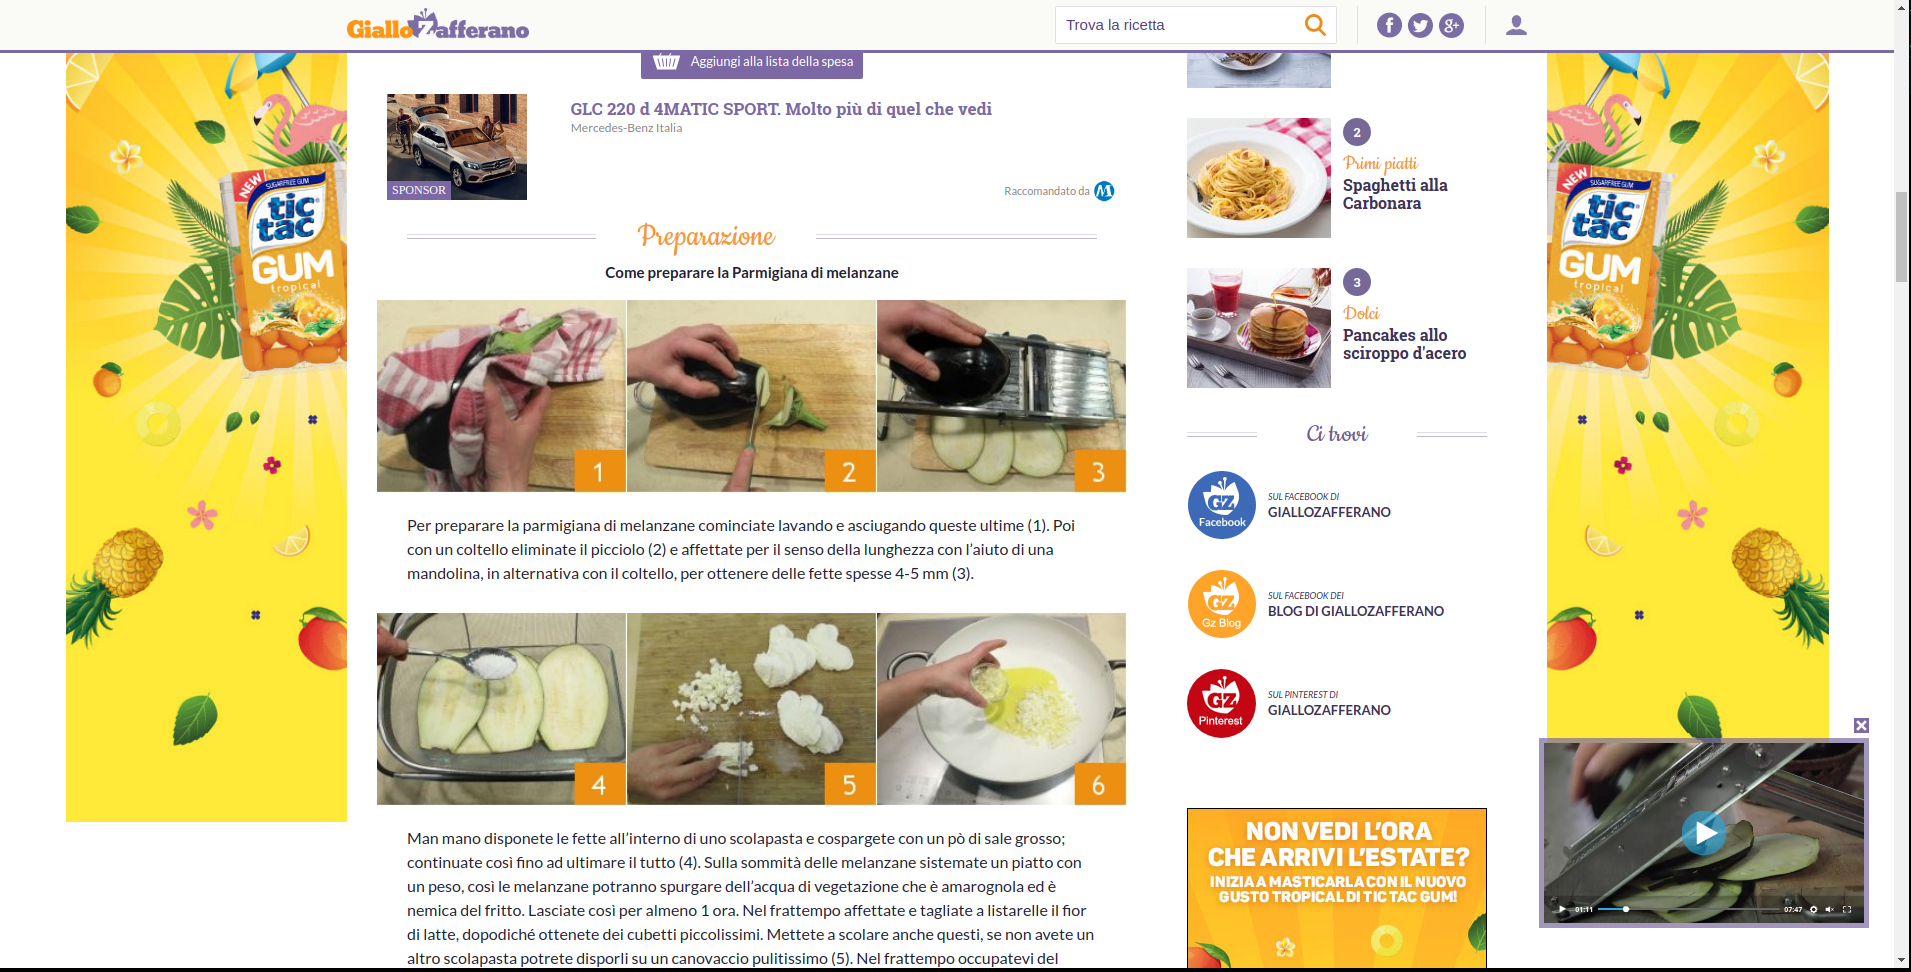
\includegraphics[scale=0.2]{images/ricetta-3.png}}
	\caption{Terza schermata della pagina ricetta della parmigiana di melanzane (ricetta-3.png)-\newline https://ricette.giallozafferano.it/Parmigiana-di-melanzane.html}
	\label{fig:ricetta-3}
\end{figure}

La successiva sezione ha come titolo \textit{Preparazione} ed è la parte più importante della ricetta; è presente un sottotitolo "Come preparare la Parmigiana di melanzane", scritto in grassetto, il quale può aiutare nella fase di scan ad identificare la sezione, qualora il titolo (che ricordo è poco leggibile perchè scritto in corsivo) non venga notato/letto. 
Ogni ricetta ha una struttura comune: il procedimento viene descritto tramite dei paragrafi di testo separati da serie di immagini, alle quali il testo fa riferimento; nonostante sia una scelta che sicuramente facilita la comprensione del procedimento, le immagini continuano a non essere cliccabili, il che comporta gli stessi problemi di cui ho parlato sotto a \ref{fig:ricetta-2}. Inoltre, è buona cosa che il testo sia diviso in blocchi, ma in esso non è presente alcuna parola chiave evidenziata, nè un titolo descrittivo: per quanto riguarda quest'ultimo, esso può non servire in questo particolare caso, dato che i blocchi sono strettamente collegati, invece le keywords mancanti sono un errore che sfavorisce lo scanning.

\clearpage

\begin{figure}[h!]
	\centerline{
	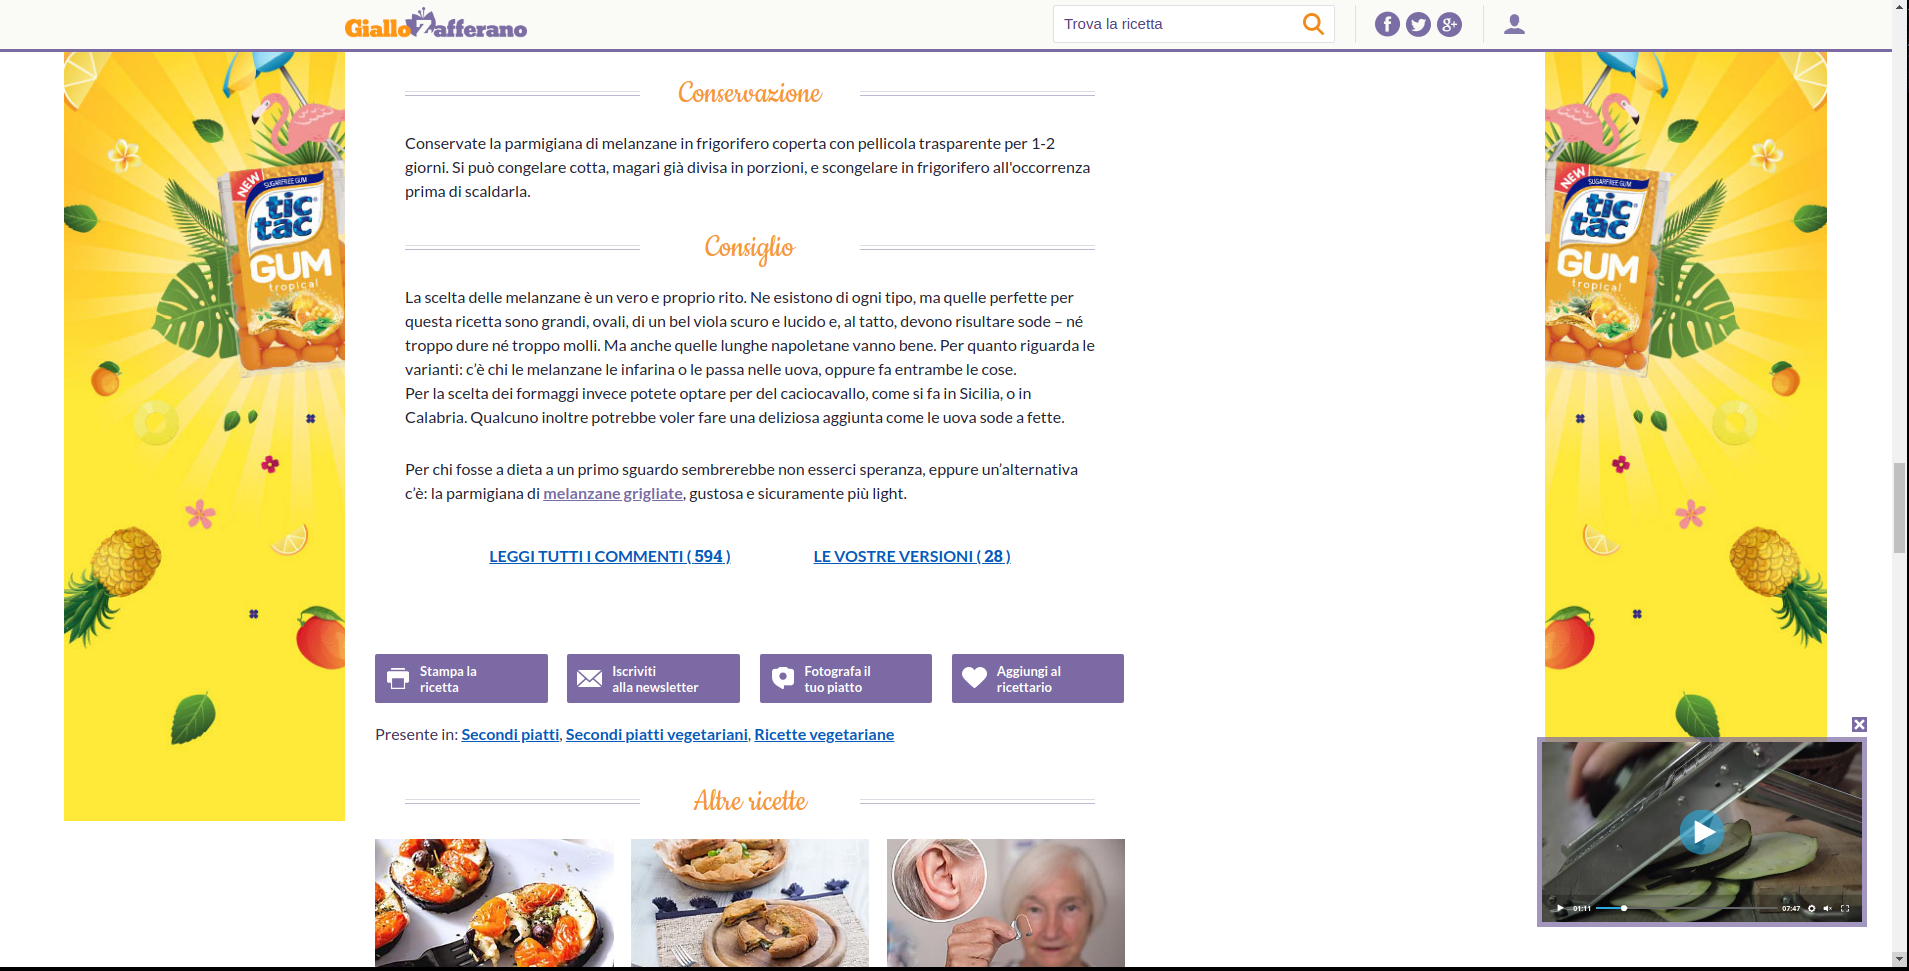
\includegraphics[scale=0.2]{images/ricetta-6.png}}
	\caption{Sesta schermata della pagina ricetta della parmigiana di melanzane (ricetta-6.png) -\newline https://ricette.giallozafferano.it/Parmigiana-di-melanzane.html}
	\label{fig:ricetta-6}
\end{figure}

Saltiamo qualche schermata dato che quarta e quinta sono identiche alla terza. Qui vediamo tre blocchi di testo abbastanza sintetici, dei quali il primo è da solo sotto il titolo \textit{Conservazione} e specifica le modalità di conservazione della pietanza, mentre gli altri due stanno sotto il titolo \textit{Consiglio}, dove vengono dati consigli relativi a questioni specifiche della ricetta. Alla luce del loro contenuto, possiamo dire che la posizione (alla fine) è  perfetta, perché sono informazioni aggiuntive di cui non tutti possono aver bisogno.
I vari blocchi facilitano lo scanning e in questo particolare caso, aver linkato \textit{melanzane grigliate}, attira sicuramente l'attenzione dell'utente.
In seguito sono presenti vari link, la maggior parte dei quali verrà probabilmente ignorata.
Notiamo poi la presenza di un accenno di breadcrumb: "\textit{presente in: secondi piatti, secondi piatti vegetariani, ricette vegetariane}" aiuta sicuramente a capire meglio la struttura e i percorsi di navigazione all'interno del sito, ma la scelta di posizionarlo così in basso è un grave errore e ne dà pochissima visibilità e quindi utilità.
\clearpage

\begin{figure}[h!]
	\centerline{
	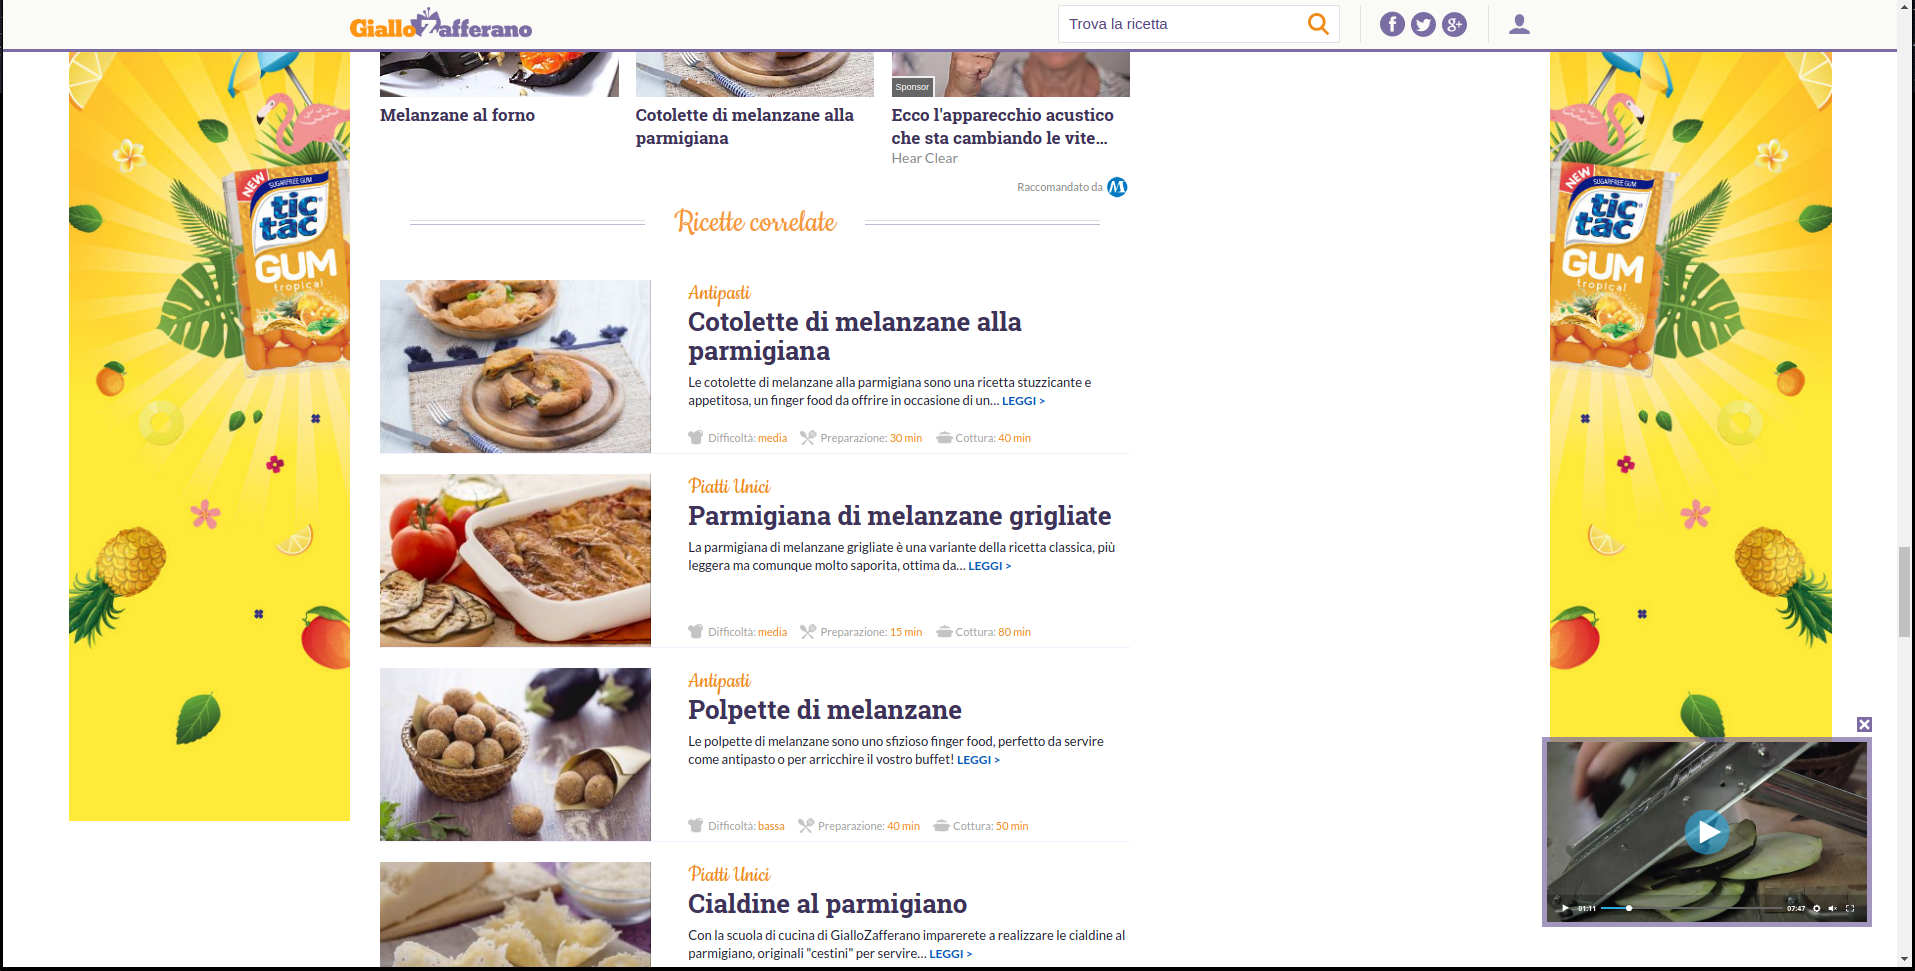
\includegraphics[scale=0.2]{images/ricetta-7.png}}
	\caption{Settima schermata della pagina ricetta della parmigiana di melanzane (ricetta-7.png) -\newline https://ricette.giallozafferano.it/Parmigiana-di-melanzane.html}
	\label{fig:ricetta-7}
\end{figure}

\begin{figure}[h!]
	\centerline{
	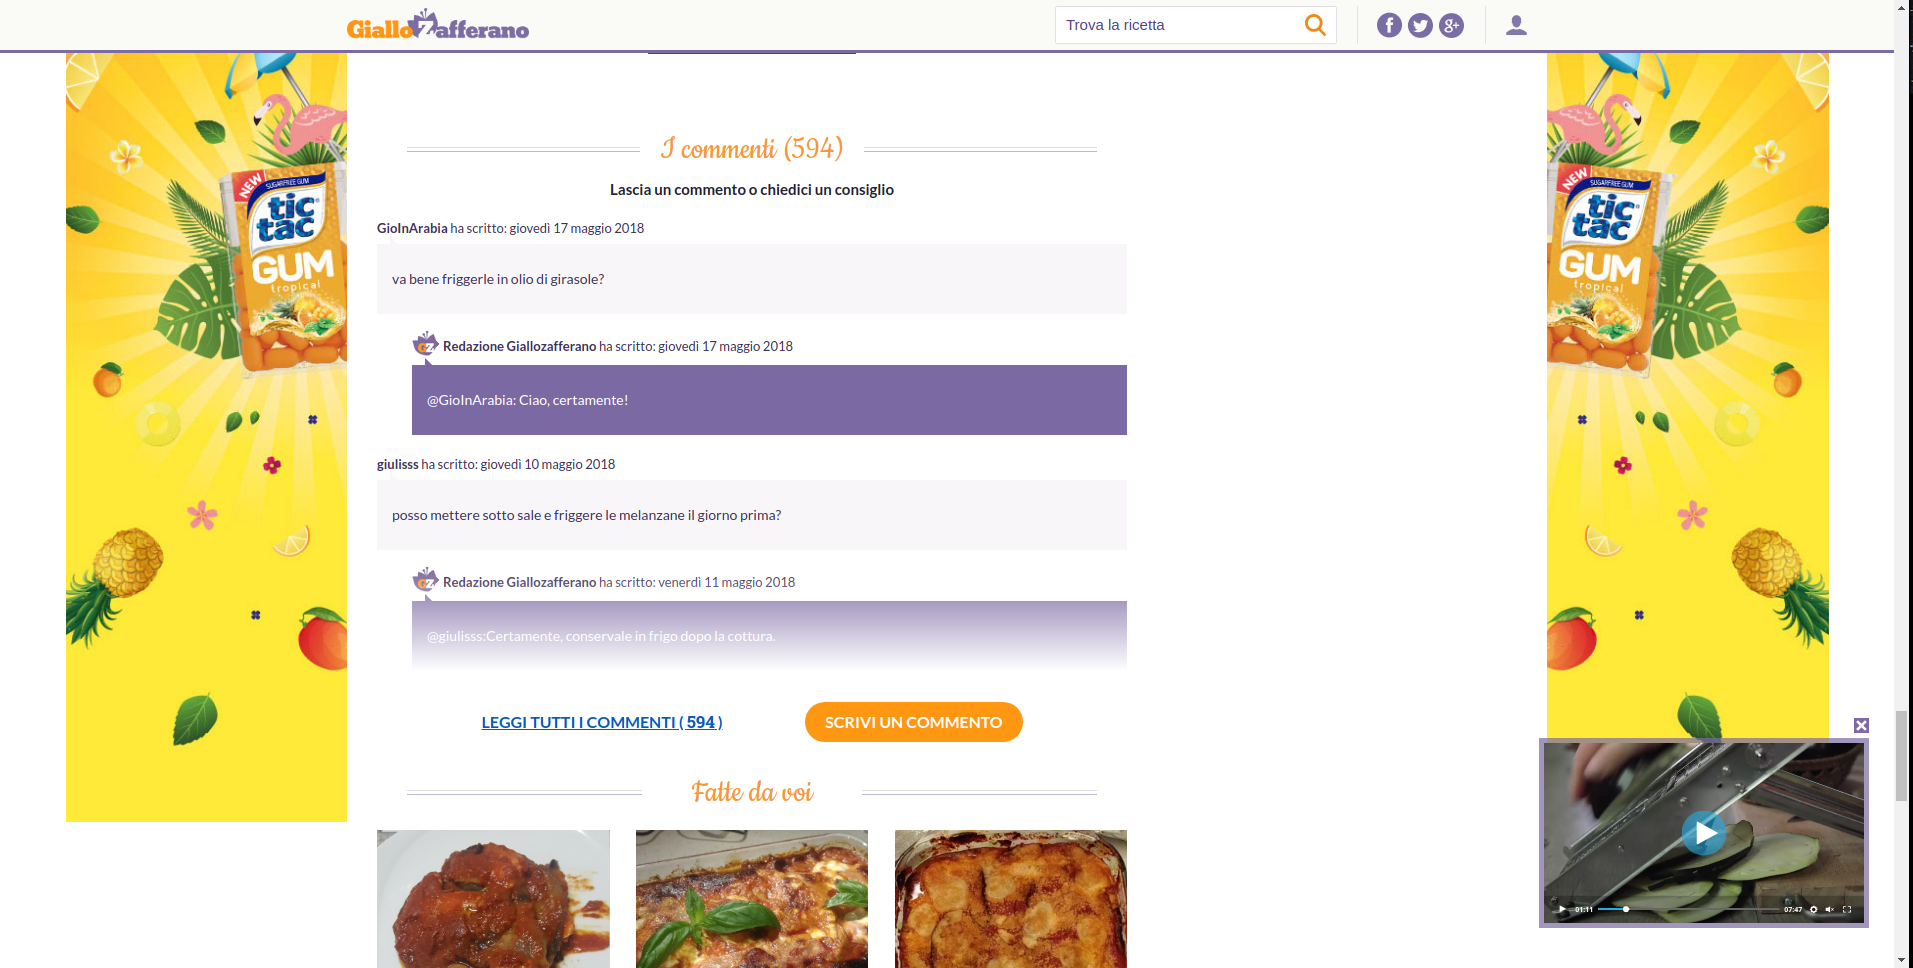
\includegraphics[scale=0.2]{images/ricetta-8.png}}
	\caption{Ottava schermata della pagina ricetta della parmigiana di melanzane (ricetta-8.png) -\newline https://ricette.giallozafferano.it/Parmigiana-di-melanzane.html}
	\label{fig:ricetta-8}
\end{figure}

In seguito vediamo la sezione "\textit{Altre ricette}" (per metà in figura \ref{fig:ricetta-6}), in cui vengono posti riferimenti ad altre ricette all'interno del sito, cosa che può invogliare l'utente a non abbandonare il sito; sono presentate come immagini disposte a griglia, cosa che permette di visualizzare più informazione in maniera compatta, anche se manda in crisi la fase di scan. 
Subito dopo appare la sezione "\textit{Ricette correlate}",che presenta ulteriori riferimenti a ricette presenti nel sito: a differenza della sezione precedente, però, l'informazione viene presentata con un layout a lista, il che può confondere l'utente, in quanto incoerente con il layout della sezione precedente.
Appena sotto c'è la sezione commenti, che finalmente riesce a dare al sito un senso di dinamicità ed aggiornamento, oltre a coinvolgere attivamente gli utenti.
Per finire, sono presenti molti altre sezioni di riferimenti a parti del sito, ma non mi ci soffermerò in quanto finirei per ripetermi. Una cosa a cui porre attenzione è invece la presenza di una barra di ricerca alla fine di tutti il contenuto: ad essa è riservata un'intera riga, tuttavia la posizione la svantaggia fortemente, dato che sicuramente sarà vista da un numero esiguo di utenti poiché, come detto in precedenza,la pagina si compone di moltissimi scroll.

\subsection{404}

\begin{figure}[h!]
	\centerline{
	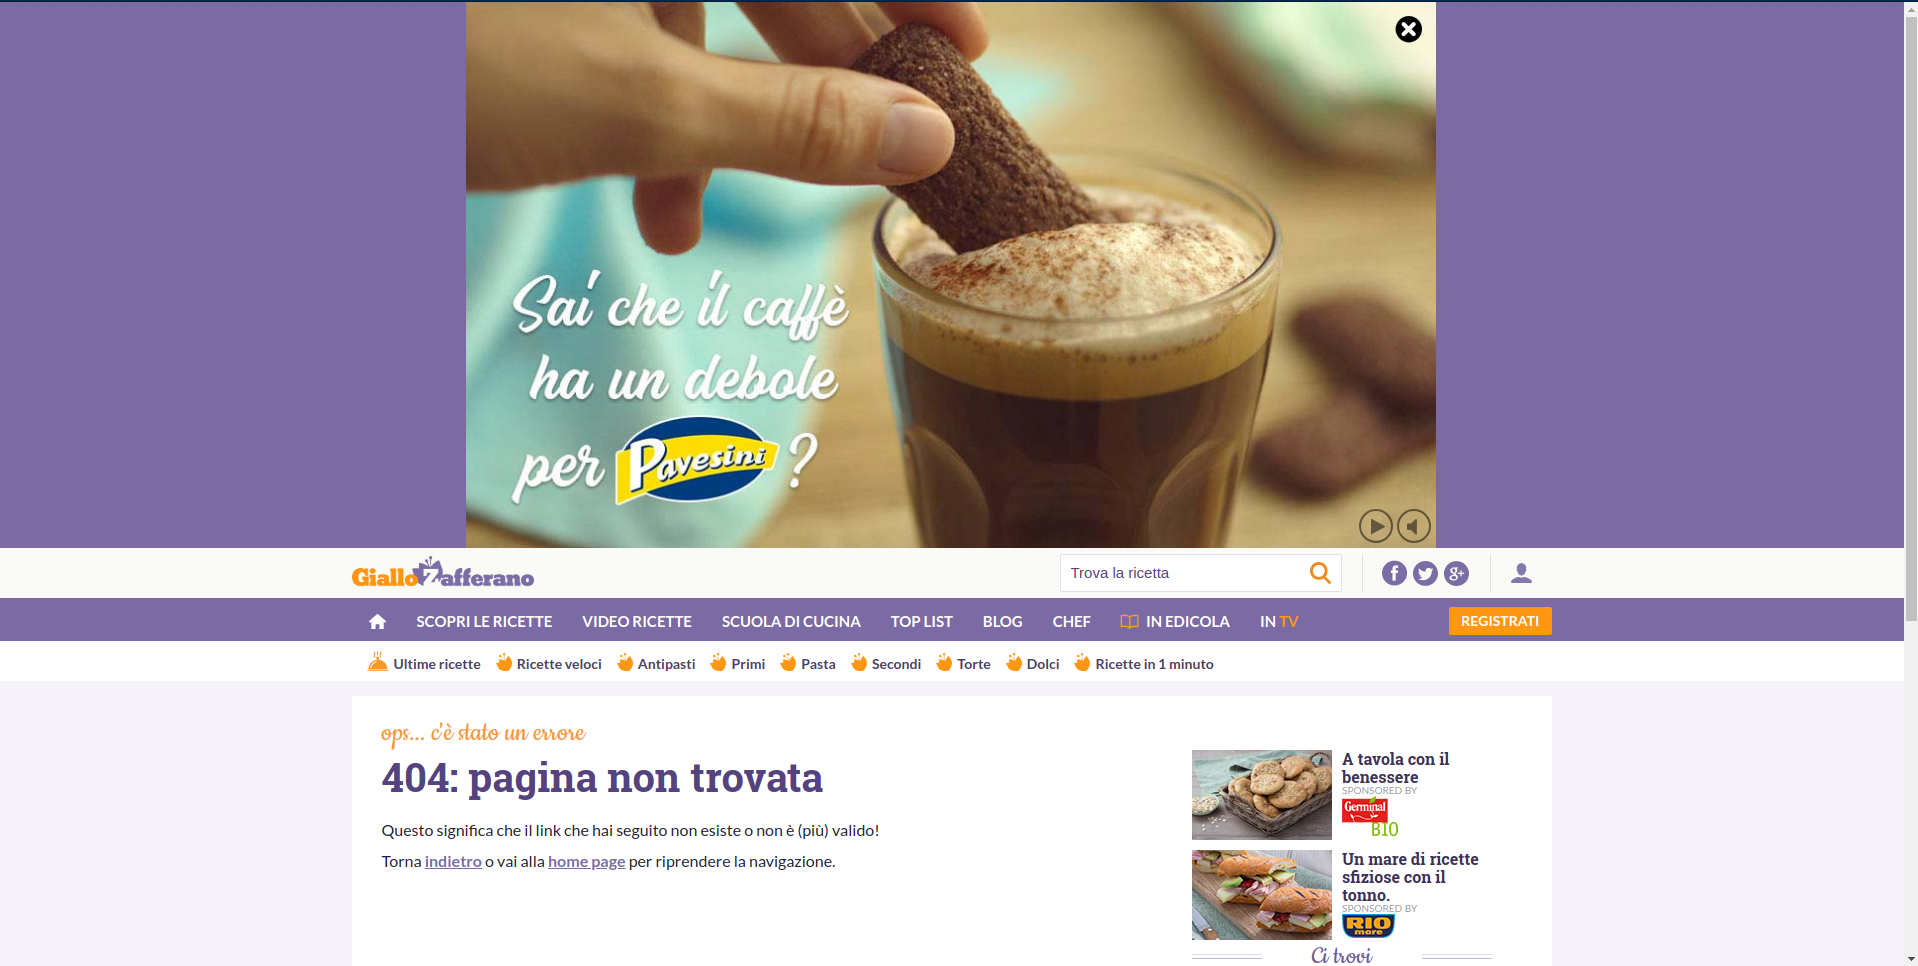
\includegraphics[scale=0.2]{images/404.png}}
	\caption{Pagina non trovata (404.png) - https://ricette.giallozafferano.it/asdasd}
	\label{fig:404}
\end{figure}

Quando l'utente medio finisce in una pagina inesistente, egli necessita di spiegazioni semplici, senza uso di tecnicismi; giallozafferano si comporta abbastanza bene, innanzitutto vediamo la scritta "\textit{ops...c'è stato un errore}", seguita dal titolo "\textit{404: pagina non trovata}". L'utilizzo del codice 404 è sconsigliato, in quanto è puramente tecnico e, nonostante molti utenti siano a conoscenza del loro significato, mediamente c'è il rischio che provochi confusione nel visitatore. Il paragrafo che segue dà però una spiegazione sintetica e comprensibile dell'errore, fornendo all'utente dei link alla home page o a alla pagina precedente: quest'ultima cosa è tuttavia rischiosa, poiché se il visitatore era arrivato alla pagina tramite il deep linking, farlo tornare indietro significherebbe farlo uscire dal sito e inoltre, nel caso in cui il visitatore avesse \textit{javascript} disattivato, tale link non avrebbe alcuna conseguenza e accrescerebbe la frustrazione dell'utente che sia aspetta un reindirizzamento.
\section{Strumenti: ricerca}
Giallozafferano è un sito web contenente moltissima informazione, divisa in tantissime pagine raggruppate in sezioni; la ricerca è dunque uno strumento fondamentale e necessario anche per risolvere il problema della \textbf{long tail}, cioè il fenomeno per cui solo poche pagine ottengono circa l'80\% dell'attenzione. Si stima inoltre che la ricerca venga utilizzata circa nel 60\% dei casi di deep linking, dato che gli utenti sono abituati ai motori di ricerca.
Il sito in esame è inoltre frequentemente aggiornato, è dunque cruciale l'utilizzo di un buon motore di ricerca, dato che spesso i menù da soli non riescono a seguire gli aggiornamenti.
\\~\textbf{Premessa}: quando si è analizzata la pagina della ricetta, si è fatto notare la presenza di una barra di ricerca alla fine di tale pagina; dato che essa è presente solo in quella tipologia di pagina e come detto sarà vista da pochissimi utenti, si è deciso di non considerarla.
\\~Come si può vedere in una qualsiasi delle schermate presenti nelle sezioni precedenti, la ricerca è posizionata in alto a destra, posizione perfetta. Essa è composta da un box testuale che supporta un numero massimo di 26 caratteri prima che uno di essi venga nascosto: non sono molti, ma potrebbero essere sufficienti a soddisfare una percentuale abbastanza elevata di utenti (con 30 caratteri è soddisfatto circa l'80\% degli utenti); la grandezza del search box è fondamentale, poiché per ogni carattere nascosto aumenta proporzionalmente lo stress e l'utente medio tende inconsciamente a rimanere entro il limite imposto, scrivendo query meno specifiche che portano a risultati più scarsi. Visto lo spazio a disposizione, sarebbe stato più saggio utilizzare un box dinamico che aumenta in grandezza non appena l'utente vi clicca sopra.
\\~Altro punto fondamentale è il pulsante di ricerca: giallozafferano opta per l'utilizzo del simbolo della lente di ingrandimento, cosa abbastanza popolare nel web ma più adatta ad un sito mobile: ancora una volta, vista la quantità di spazio a disposizione, sarebbe stato meglio utilizzare un pulsante con scritto "\textit{cerca}" o "\textit{search}".

\subsection{Pagina dei risultati}

\begin{figure}[h!]
	\centering
	\begin{subfigure}[b]{0.4\textwidth}
		
\includegraphics[scale=0.1]{images/risultati/risultati-0.jpeg}
		\subcaption{}
	\end{subfigure}
	\begin{subfigure}[b]{0.4\textwidth}
		
\includegraphics[scale=0.1]{images/risultati/risultati-1.jpeg}
		\subcaption{}
	\end{subfigure}
	\begin{subfigure}[b]{0.4\textwidth}
		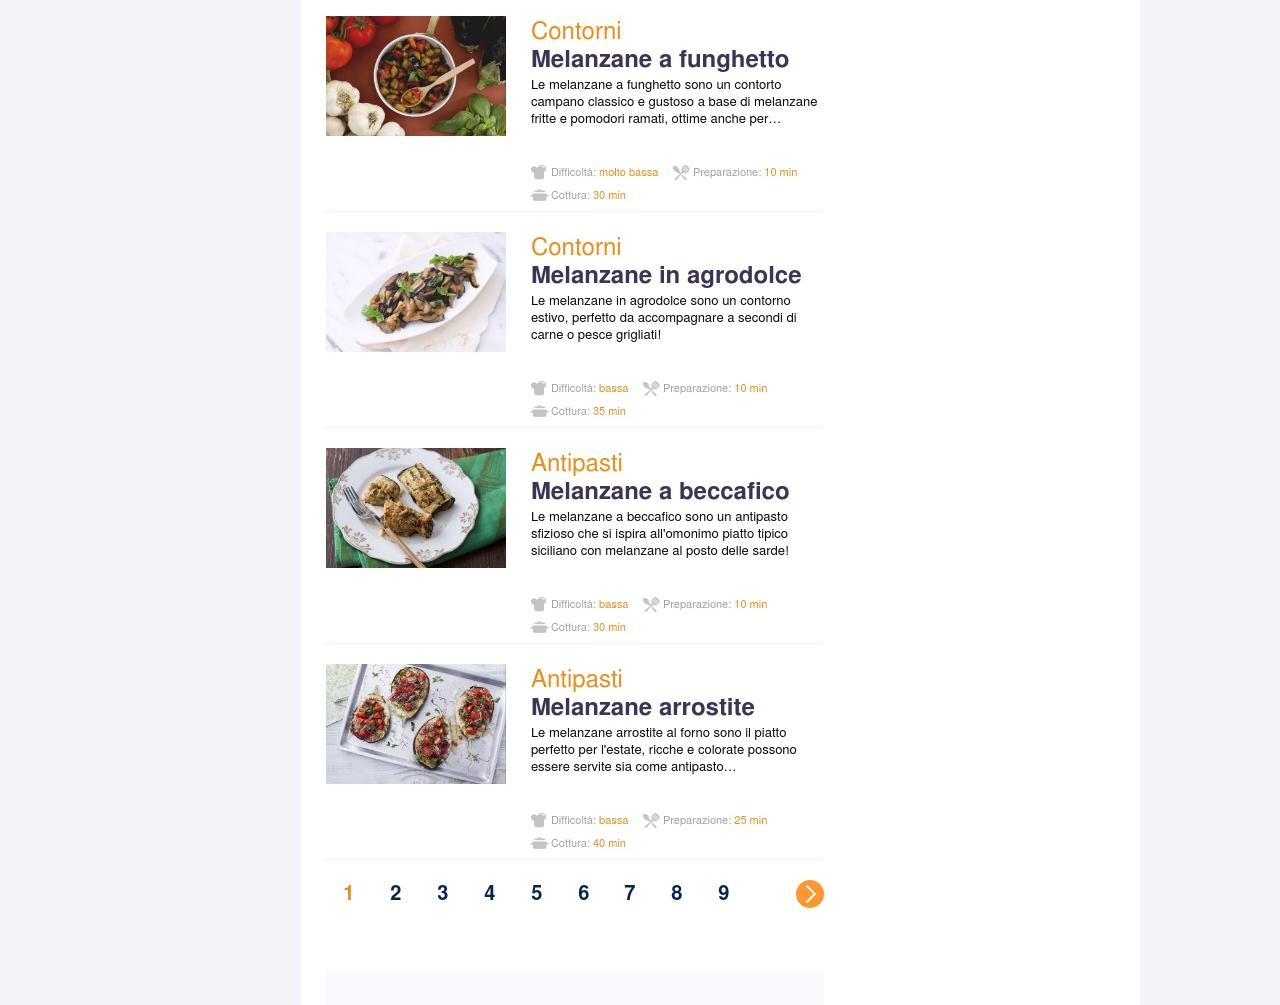
\includegraphics[scale=0.1]{images/risultati/risultati-2.jpeg}
		\subcaption{}
	\end{subfigure}
	\caption{Pagina dei risultati della query "melanzane" (risultati-0,1,2.png) -\newline https://www.giallozafferano.it/ricerca-ricette/melanzane/}
	\label{fig:risultati}
\end{figure}

Le immagini precedenti mostrano la pagina a cui si viene rimandati nel momento in cui si effettua una ricerca: notiamo che come prima cosa viene specificato il numero di risultati trovati, con la sintassi "\textit{Numero ricette: query}"; ciò è sicuramente un'informazione importante, soprattutto nel caso di 0 risultati, poiché chiarisci all'utente se la ricerca è andata a buon fine oppure no.
I risultati vengono presentati in lista: ciò permette di specificare più informazioni riguardo ogni singolo risultato, tuttavia fa un cattivo uso dello spazio, allungandosi in verticale e dividendo i risultati in molte pagine diverse; l'utilizzo di una griglia, in questo caso, sarebbe stata la scelta migliore perché avrebbe compattato l'informazione, permettendo una visualizzazione di più risultati in meno spazio. 
Un'altra cosa che manca è l'aggiunta della ricerca vincolata: dato che le ricette possono essere divise (e sono divise all'interno del sito) in categorie diverse, viene naturale pensare all'introduzione di filtri di ricerca, che aiuterebbero l'utente a trovare esattamente ciò che gli interessa, soprattutto in caso di molti risultati.
Manca anche una possibilità di ordinamento, cosa che costringe l'utente a scrollare e andare avanti nelle pagine per cercare ciò che vuole. 



\section{Pubblicità}
Giallozafferano è tempestato di pubblicità, tanto da riservarvi una quantità di spazio quanta quella relativa ai contenuti: è perfettamente normale che un sito web sfrutti gli annunci per guadagnare, ma è necessario tenere a mente che l'obiettivo principale deve essere fornire correttamente informazione agli utenti del sito.
In generale le pubblicità all'interno del sito sono abbastanza correlate al cibo, tuttavia spesso è possibile incontrarne di completamente scorrelate, cosa che distrae l'utente abbassandone i timer e abbassa la sua voglia di tornare.
Come si può vedere in \ref{fig:homepage}, l'intera homepage ha pubblicità nel suo contenuto, ma in questo caso il sito la posiziona abbastanza bene: innanzitutto ne vediamo nella colonna di destra, posizione in cui gli utenti rivolgono poco lo sguardo, ma non la peggiore (fine della pagina); è poi interessante osservare come si cerchi di fondere contenuto e annunci, attraverso la tecnica del \textit{blending}: vengono presentate delle ricette interne al sito ma sponsorizzate da vari marchi, in modo da non far capire all'utente che si trattano in realtà di pubblicità (la loro URL inizia con https://adclick...). Si veda la figura sottostante (\ref{fig:blending}).

\begin{figure}[h!]
	\centering
	
\includegraphics[scale=0.2]{images/blending.png}
	\caption{Pubblicità nella homepage - blending}
	\label{fig:blending}
\end{figure}

Altri esempi di pubblicità all'interno del sito si possono vedere nella prossima schermata (figura \ref{fig:pubblicita}).
Vediamo che la pubblicità viene posta dietro al contenuto, al posto dello sfondo: è una buona posizione perché non copre informazione, tuttavia è persistente ed un utente costretto a vederla in continuazione senza avere le possibilità di chiuderla e potrebbe infastidirsi.
Un grave errore di usabilità è quello che si vede nella parte alta della schermata: un video pubblicitario che parte in automatico. Innanzitutto non è coerente con il resto del sito, perché è presente solo ogni tanto e in determinate pagine; in seguito, come detto per la pagina di una ricetta, un video non dovrebbe mai partire in automatico, anche se senza volume. Come ultima cosa, poi, non permette di essere chiuso: alla luce di tutti questi problemi, risulta chiaro come una scelta del genere possa diminuire fortemente il tasso di usabilità del sito.

\begin{figure}[h!]
	\centering
	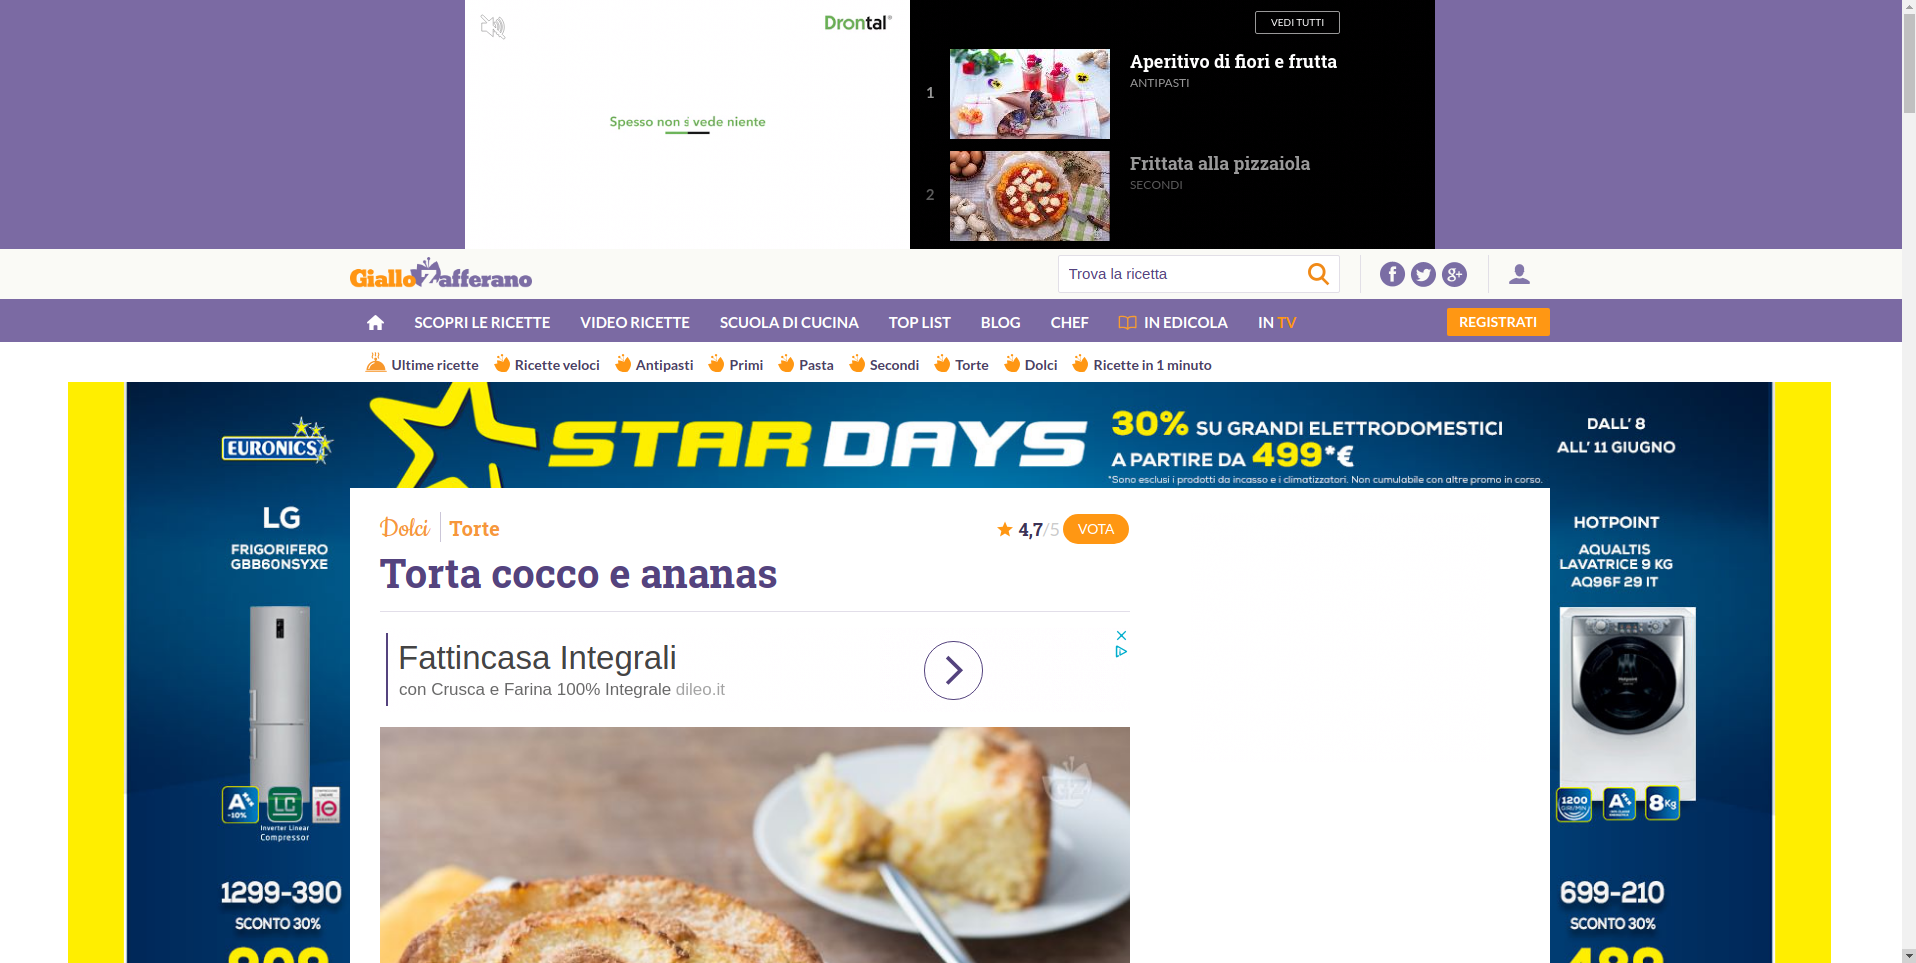
\includegraphics[scale=0.2]{images/pubblicita.png}
	\caption{Pubblicità (pubblicità.png)}
	\label{fig:pubblicita}
\end{figure}



\section{Valutazione}
Alla luce di tutte le considerazioni fatte nel documento, giallozafferano è in grado di fornire i propri contenuti ad utenti di tutti i tipi, ma nel complesso è disorganizzato e confusionario e, come visto, commette alcuni gravi errori di usabilità: per questo il voto che merita secondo me è \textbf{6/10}.

\end{document}